%  LaTeX support: latex@mdpi.com
%=================================================================
\documentclass[data,datadescriptor,submit,pdftex,moreauthors]{Definitions/mdpi}

%--------------------
% Class Options:
%   data            - Data journal
%   datadescriptor  - Data Descriptor article type
%   submit          - Line numbers on (changed to "accept" by editorial office)
%   pdftex          - For pdfLaTeX compilation
%   moreauthors     - Multiple authors
%--------------------

%=================================================================
% MDPI internal commands - do not modify
\firstpage{1}
\makeatletter
\setcounter{page}{\@firstpage}
\makeatother
\pubvolume{1}
\issuenum{1}
\articlenumber{0}
\pubyear{2026}
\copyrightyear{2026}
\datereceived{ }
\daterevised{ }
\dateaccepted{ }
\datepublished{ }

%=================================================================
% Additional packages
\usepackage{url}
\usepackage{tikz}
\usetikzlibrary{arrows.meta, positioning, fit, backgrounds}

%=================================================================
% Title
\Title{UML-in-the-Wild: A Dataset of UML Diagrams in PlantUML Notation from Open-Source Repositories}

% Author ORCID IDs
\newcommand{\orcidauthorA}{0009-0000-2161-4560}
\newcommand{\orcidauthorB}{0000-0000-0000-000X} % TODO: Add ORCID

% Authors
\Author{Volodymyr Polischuk $^{1,}$*\orcidA{} and Firstname Lastname $^{1}$\orcidB{}}

% Affiliations
\address{%
$^{1}$ \quad Kyiv National University of Technologies and Design, 01011 Kyiv, Ukraine}

% Corresponding author
\corres{Correspondence: polishchuk.vl@knutd.edu.ua}

%=================================================================
% Abstract
\abstract{%
% ~200 words, single paragraph, no citations, no headings.
% Structure (without labels): Background, Methods, Results, Conclusions.
UML diagrams are widely used in software engineering, yet large-scale empirical datasets remain scarce. We present UML-in-the-Wild, a dataset of 143,427 UML diagrams extracted from open-source repositories via the World of Code infrastructure. The pipeline identifies PlantUML files by extension across 128 basemap shards, validates content markers, compiles diagrams using PlantUML, and classifies them into 9 standard UML types using an LLM-based classifier. The dataset spans class (51.6\%), sequence (24.6\%), activity (6.8\%), component (5.7\%), use case (5.0\%), state (3.0\%), object (1.7\%), deployment (1.4\%), and timing (0.1\%) diagrams. Each diagram is provided as both PlantUML source and rendered PNG, accompanied by metadata including diagram type, structural element and connection counts, and source repository attribution. UML-in-the-Wild is the largest publicly available collection of real-world UML diagrams, enabling research in software engineering, model-driven engineering, and AI-based diagram analysis.}

% Keywords
\keyword{UML diagrams; PlantUML; software engineering; open-source; dataset; World of Code; diagram classification}

%=================================================================
% Dataset fields (required for Data journal)
\dataset{DOI: \url{https://doi.org/10.5281/zenodo.18952372}}
\datasetlicense{CC-BY-4.0}

%=================================================================
\begin{document}

%%%%%%%%%%%%%%%%%%%%%%%%%%%%%%%%%%%%%%%%%%
\section{Summary}
\label{sec:summary}

The Unified Modeling Language (UML) has been the dominant standard for software modeling since its adoption by the Object Management Group in 1997. Despite its central role in software engineering curricula and industry practice, empirical knowledge about real-world UML usage remains limited. Although earlier surveys suggested declining adoption---Petre~\cite{petre2013uml} reported that many professional developers prefer informal notations over UML---recent evidence paints a more nuanced picture. Reggio et al.~\cite{reggio2014who} found that class, sequence, state, and activity diagrams remain widely known and used across both industry and academia, while Romeo et al.~\cite{romeo2025uml} observed that UML usage in open-source projects has been growing steadily. In open-source software specifically, Ho-Quang et al.~\cite{hoquang2017practices} identified collaboration as the primary motivation for UML use, particularly for onboarding new contributors.

A key obstacle to advancing empirical research on UML is the scarcity of large-scale, openly available datasets of real-world diagrams. While large-scale open-source mining infrastructures such as the World of Code (WoC)~\cite{ma2021world}---which indexes repositories from GitHub, GitLab, Bitbucket, and other forges---now provide comprehensive coverage of the open-source ecosystem, no prior study has leveraged such resources to systematically extract UML diagrams.

Several efforts have been made to address this gap. Karasneh and Chaudron~\cite{karasneh2013img2uml} created the Img2UML repository with approximately 1000 class models in XMI format extracted from web sources. The Lindholmen dataset~\cite{hebig2016quest,robles2017extensive}, the largest prior collection, comprises over 93,000 UML files mined from GitHub in image, XMI, and textual formats, but does not classify diagrams by type and does not include PlantUML files. A subsequent reflection by Robles et al.~\cite{robles2023reflection} discussed lessons learned from the Lindholmen dataset, noting that format heterogeneity and the absence of structured metadata posed challenges for downstream research. More recently, Romeo et al.~\cite{romeo2025uml} studied UML evolution across 552 GitHub repositories, identifying 9875 UML files in 29 different formats including PlantUML, with selection criteria (projects with over 2000 commits, 100 stars, and 10 contributors) targeting well-established projects. Notably, their findings confirm that PlantUML is the most prevalent UML format by file extension in contemporary open-source projects. St\"{o}rrle et al.~\cite{storrle2014index} documented a broader problem: of 12 reported model corpora, only 5 were active at the time of their survey, highlighting the fragility of research datasets in this domain.

At the same time, the demand for UML diagram data has grown substantially with the rise of machine learning applications in software engineering. Recent work has applied convolutional neural networks~\cite{gosala2021classification} and vision transformers~\cite{groundtruth2024} to UML diagram classification, but these efforts rely on small curated image datasets (2626--3282 images). Multimodal large language models have also been used to generate PlantUML code from diagram images~\cite{camara2024image,bates2025umlcodegen}, further underscoring the need for large-scale, machine-parseable UML datasets that go beyond image collections. Table~\ref{tab:dataset-comparison} compares the existing UML datasets with the dataset presented in this work.

\begin{table}[H]
\caption{Comparison of existing UML diagram datasets.\label{tab:dataset-comparison}}
\begin{tabularx}{\textwidth}{lCCCCC}
\toprule
\textbf{Dataset} & \textbf{Year} & \textbf{Size} & \textbf{Format} & \textbf{Types} & \textbf{Source} \\
\midrule
Img2UML \cite{karasneh2013img2uml}          & 2013 & 1000        & XMI             & 1        & Web \\
Lindholmen \cite{hebig2016quest,robles2017extensive} & 2016 & 93,000+     & Image, XMI      & ---       & GitHub \\
Ground Truth \cite{groundtruth2024}          & 2024 & 2626        & Image           & 6        & Curated \\
Romeo et al. \cite{romeo2025uml}             & 2025 & 9875        & Mixed           & ---      & GitHub \\
Synth. PlantUML \cite{bates2025umlcodegen}     & 2025 & $\sim$12,000 & PlantUML       & 2        & Generated \\
PFDial \cite{pfdial2025}                     & 2025 & 440         & PlantUML        & 1        & Generated \\
\textbf{UML-in-the-Wild (ours)}              & \textbf{2026} & \textbf{143,427} & \textbf{PlantUML + PNG} & \textbf{9} & \textbf{WoC} \\
\bottomrule
\end{tabularx}
\noindent{\footnotesize{Types: number of distinct UML diagram types classified. ``---'' indicates no type classification was performed. WoC: World of Code~\cite{ma2021world}.}}
\end{table}

This paper presents \emph{UML-in-the-Wild}, a dataset of 143,427 UML diagrams extracted from open-source repositories via the World of Code (WoC) infrastructure~\cite{ma2021world}. The dataset was constructed through a three-phase pipeline: (1)~extraction of PlantUML files from WoC via extension-based search and content validation, (2)~preprocessing and image generation using the PlantUML compiler, and (3)~LLM-based diagram type classification with parser-based structural analysis. Each diagram is provided in dual format---PlantUML source code and rendered PNG image---and is accompanied by rich metadata including LLM-based diagram type classification into 9 standard UML types, parser-based structural element and connection counts, textual size metrics, and source repository attribution.

The dataset differs from prior work in several key respects: (1)~it is significantly larger than any existing classified UML dataset; (2)~it is the largest collection in a textual UML notation (PlantUML), enabling direct programmatic analysis of diagram structure without image recognition; (3)~it provides per-diagram structural metrics (element and connection counts by type) that no prior dataset includes; (4)~it draws from the entire open-source ecosystem via WoC rather than a subset of GitHub repositories; and (5)~it is openly available on Zenodo under the CC-BY-4.0 license.

By publicly releasing this dataset, we aim to support several lines of research: empirical studies of how UML is used in practice across the open-source ecosystem, training and evaluation of AI models for diagram understanding and generation, analysis of diagram quality and structural complexity, and the development of educational resources for software engineering courses.

%%%%%%%%%%%%%%%%%%%%%%%%%%%%%%%%%%%%%%%%%%
\section{Data Description}
\label{sec:data-description}

% Overview of the dataset contents
The dataset comprises three components: (1)~143,427 preprocessed PlantUML diagrams (\texttt{.puml}), each containing one diagram with pipeline-injected metadata headers for provenance tracking; (2)~144,487 rendered PNG images (\texttt{.png}); and (3)~a single JSON metadata file that records diagram type, structural metrics, and provenance information for every diagram. The total size is approximately 5.3~GB, of which 625~MB corresponds to PlantUML sources, 4.6~GB to PNG images, and 116~MB to metadata. The number of rendered images exceeds the number of source files because some diagrams use PlantUML's \texttt{newpage} keyword, which produces multiple output pages---and therefore multiple PNG files---from a single source file. The subsections below describe the file organization, diagram type distribution, textual and structural metrics, metadata schema, and known limitations of the dataset.

\subsection{File Organization and Naming}
\label{sec:file-naming}

All files are named by their WoC blob identifier---a 40-character SHA-1 hex hash that uniquely identifies the file content (e.g., \texttt{5f95f42b...e89e.puml} and the corresponding \texttt{5f95f42b...e89e.png}). Files that originate from multi-diagram splitting, where a single source file contained multiple \texttt{@startuml...@enduml} blocks, use the pattern \texttt{\{blob\_id\}\_01.puml}, \texttt{\{blob\_id\}\_02.puml}, etc. Separately, diagrams that use PlantUML's \texttt{newpage} keyword produce multiple PNG images from a single source file; these follow the pattern \texttt{\{blob\_id\}\_001.png}, \texttt{\{blob\_id\}\_002.png}, etc.

Each \texttt{.puml} file begins with three pipeline-injected comment lines that record provenance information, followed by the diagram content:

\begin{verbatim}
' Blob ID: 5f95f42b5b392db1c75ab9f5c6eb514ac273e89e
' Original Path: /src/main/java/ex42/App.puml
' Source: World of Code
@startuml
...
@enduml
\end{verbatim}

\noindent These headers link each diagram back to its source repository and file path, enabling users to locate the original context. The diagram content itself preserves the original PlantUML source with two preprocessing modifications: multi-diagram files were split into individual files (see Section~\ref{sec:preprocessing}), and custom \texttt{@startuml} names were normalized to ensure consistent file naming (see Section~\ref{sec:preprocessing}).

\subsection{Diagram Type Distribution}
\label{sec:type-distribution}

Figure~\ref{fig:type-distribution} presents the distribution of diagram types in the dataset. The UML 2.5 specification defines 14 diagram types; the dataset covers 9 of these. The remaining 5 types---package, composite structure, interaction overview, communication, and profile diagrams---are not natively supported by PlantUML's diagram syntax and therefore do not appear in the source corpus.

Class diagrams dominate the dataset at 51.6\%, followed by sequence diagrams at 24.6\%; together these two types account for over three-quarters of all diagrams. This distribution is consistent with prior survey findings: Reggio et al.~\cite{reggio2014who} reported that class and sequence diagrams are the most widely known and used UML types across both industry and academia. The remaining types---activity (6.8\%), component (5.7\%), use case (5.0\%), state (3.0\%), object (1.7\%), deployment (1.4\%), and timing (0.1\%)---form a long tail, with timing diagrams being the rarest at only 189 instances.

Additionally, 983 diagrams (0.7\%) have non-empty \texttt{secondary\_types} in the metadata, indicating that they combine elements from multiple UML diagram types within a single file.

\begin{figure}[H]
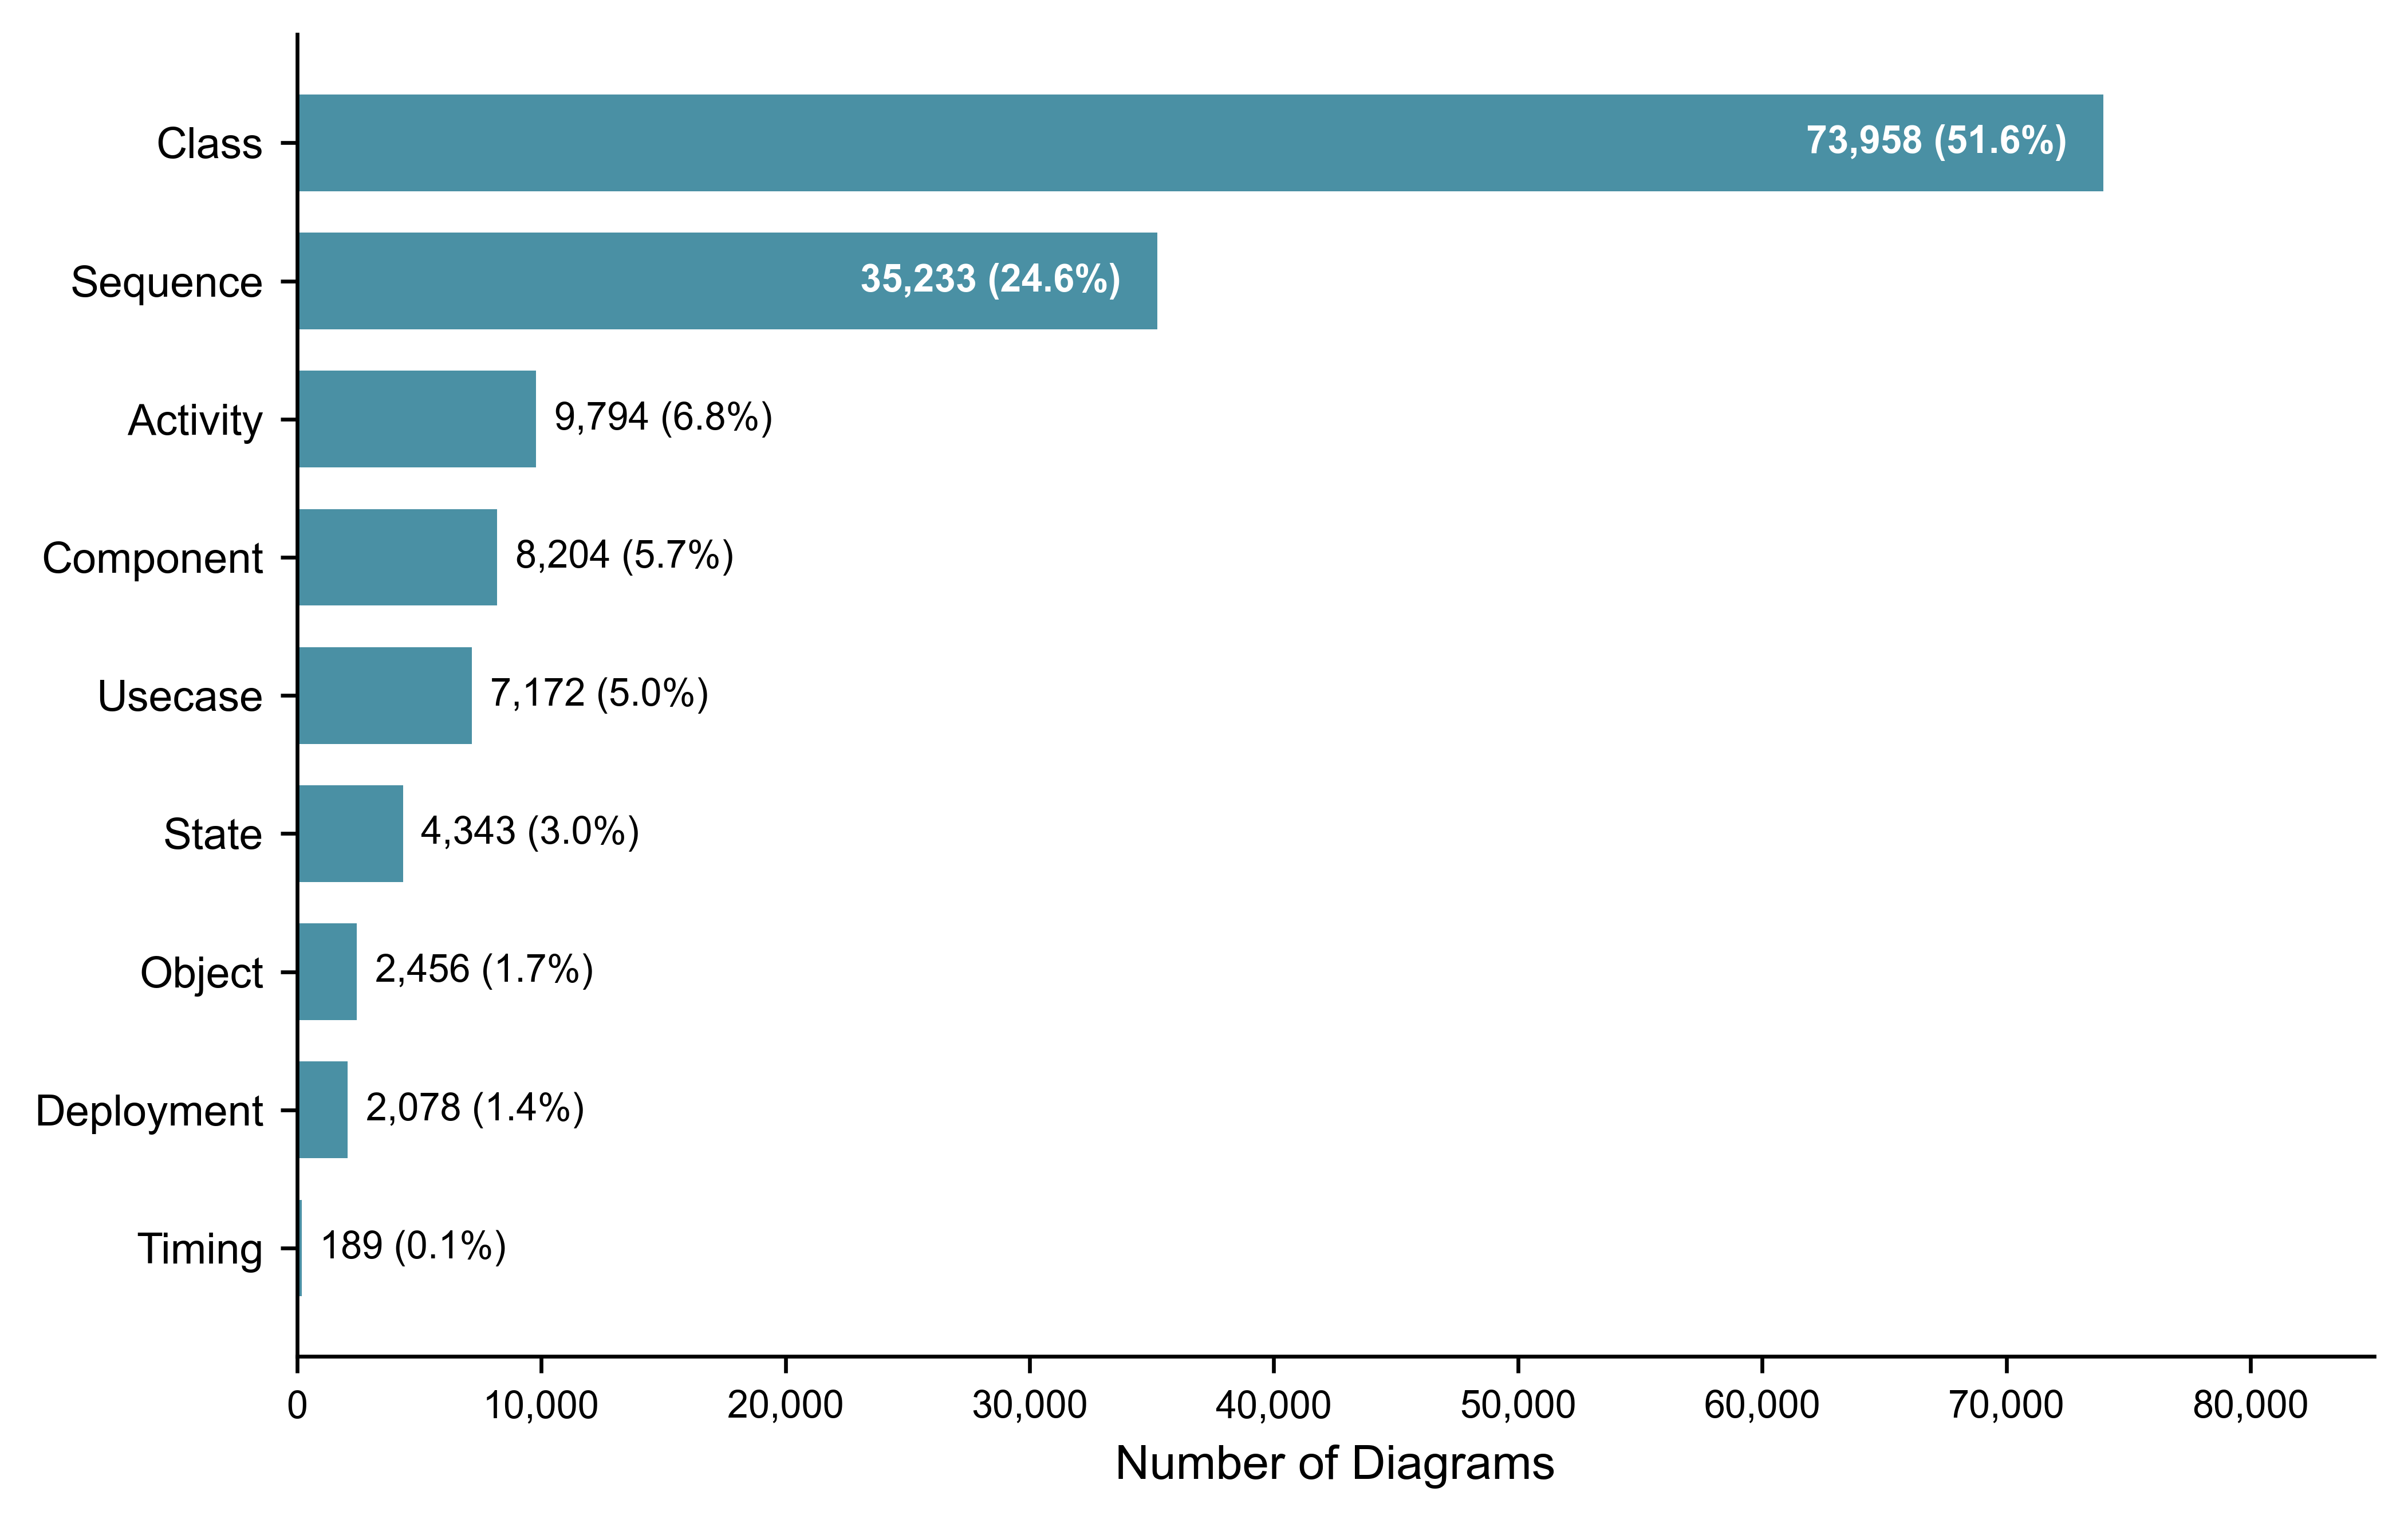
\includegraphics[width=\textwidth]{figures/fig1_type_distribution.png}
\caption{Distribution of UML diagram types in the dataset.\label{fig:type-distribution}}
\end{figure}

\subsection{Textual Size Metrics}
\label{sec:size-metrics}

We measured diagram size using \emph{content lines}---non-blank, non-comment lines excluding the pipeline-injected metadata header and \texttt{@startuml}/\texttt{@enduml} markers. Table~\ref{tab:line-distribution} shows the distribution across logarithmic bins. The distribution is right-skewed (median~=~22, mean~=~39.34, Q1~=~11, Q3~=~42, max~=~31,784), with over 93\% of diagrams containing 100 or fewer content lines.

\begin{table}[H]
\caption{Distribution of diagram size by content lines.\label{tab:line-distribution}}
\begin{tabularx}{\textwidth}{lCC}
\toprule
\textbf{Lines} & \textbf{Count} & \textbf{Percentage (\%)} \\
\midrule
1--10     & 32,870  & 22.9 \\
11--100   & 101,098 & 70.5 \\
101--1000 & 9,338   & 6.5 \\
1001+     & 121     & 0.1 \\
\bottomrule
\end{tabularx}
\end{table}

\subsection{Structural Metrics}
\label{sec:structural-metrics}

The extraction tool described in Section~\ref{sec:element-extraction} identified 1,253,248 structural elements (57 distinct types) and 1,438,155 connections (28 types) across the 143,080 successfully processed diagrams. Per-diagram element counts have a median of 6 (Q1~=~3, Q3~=~10, max~=~2,289); connection counts have a median of 6 (Q1~=~2, Q3~=~12, max~=~10,923).

Figures~\ref{fig:element-types} and~\ref{fig:connection-types} show the 15 most frequent element and connection types, respectively. The most common elements are classes (35.4\%), packages (12.6\%), and sequence diagram participants (10.4\%); the most common connections are sequence diagram messages (32.0\%), generic directed associations (25.5\%), and inheritance relationships (14.7\%). Type labels are derived from PlantUML's internal parser data model rather than standard UML vocabulary---for example, \texttt{simple} denotes an activity diagram action node, and \texttt{description} encompasses component and deployment entities. Section~\ref{sec:element-extraction} describes the label semantics and extraction strategies in detail.

Of the 143,427 diagrams in the dataset, 347 (0.2\%) could not be processed by the extraction tool, resulting in empty element and connection fields. These failures are predominantly timing diagrams (178) and multi-page diagrams using the \texttt{newpage} keyword (167). The \texttt{extraction\_error} field in the metadata identifies all affected records.

\begin{figure}[H]
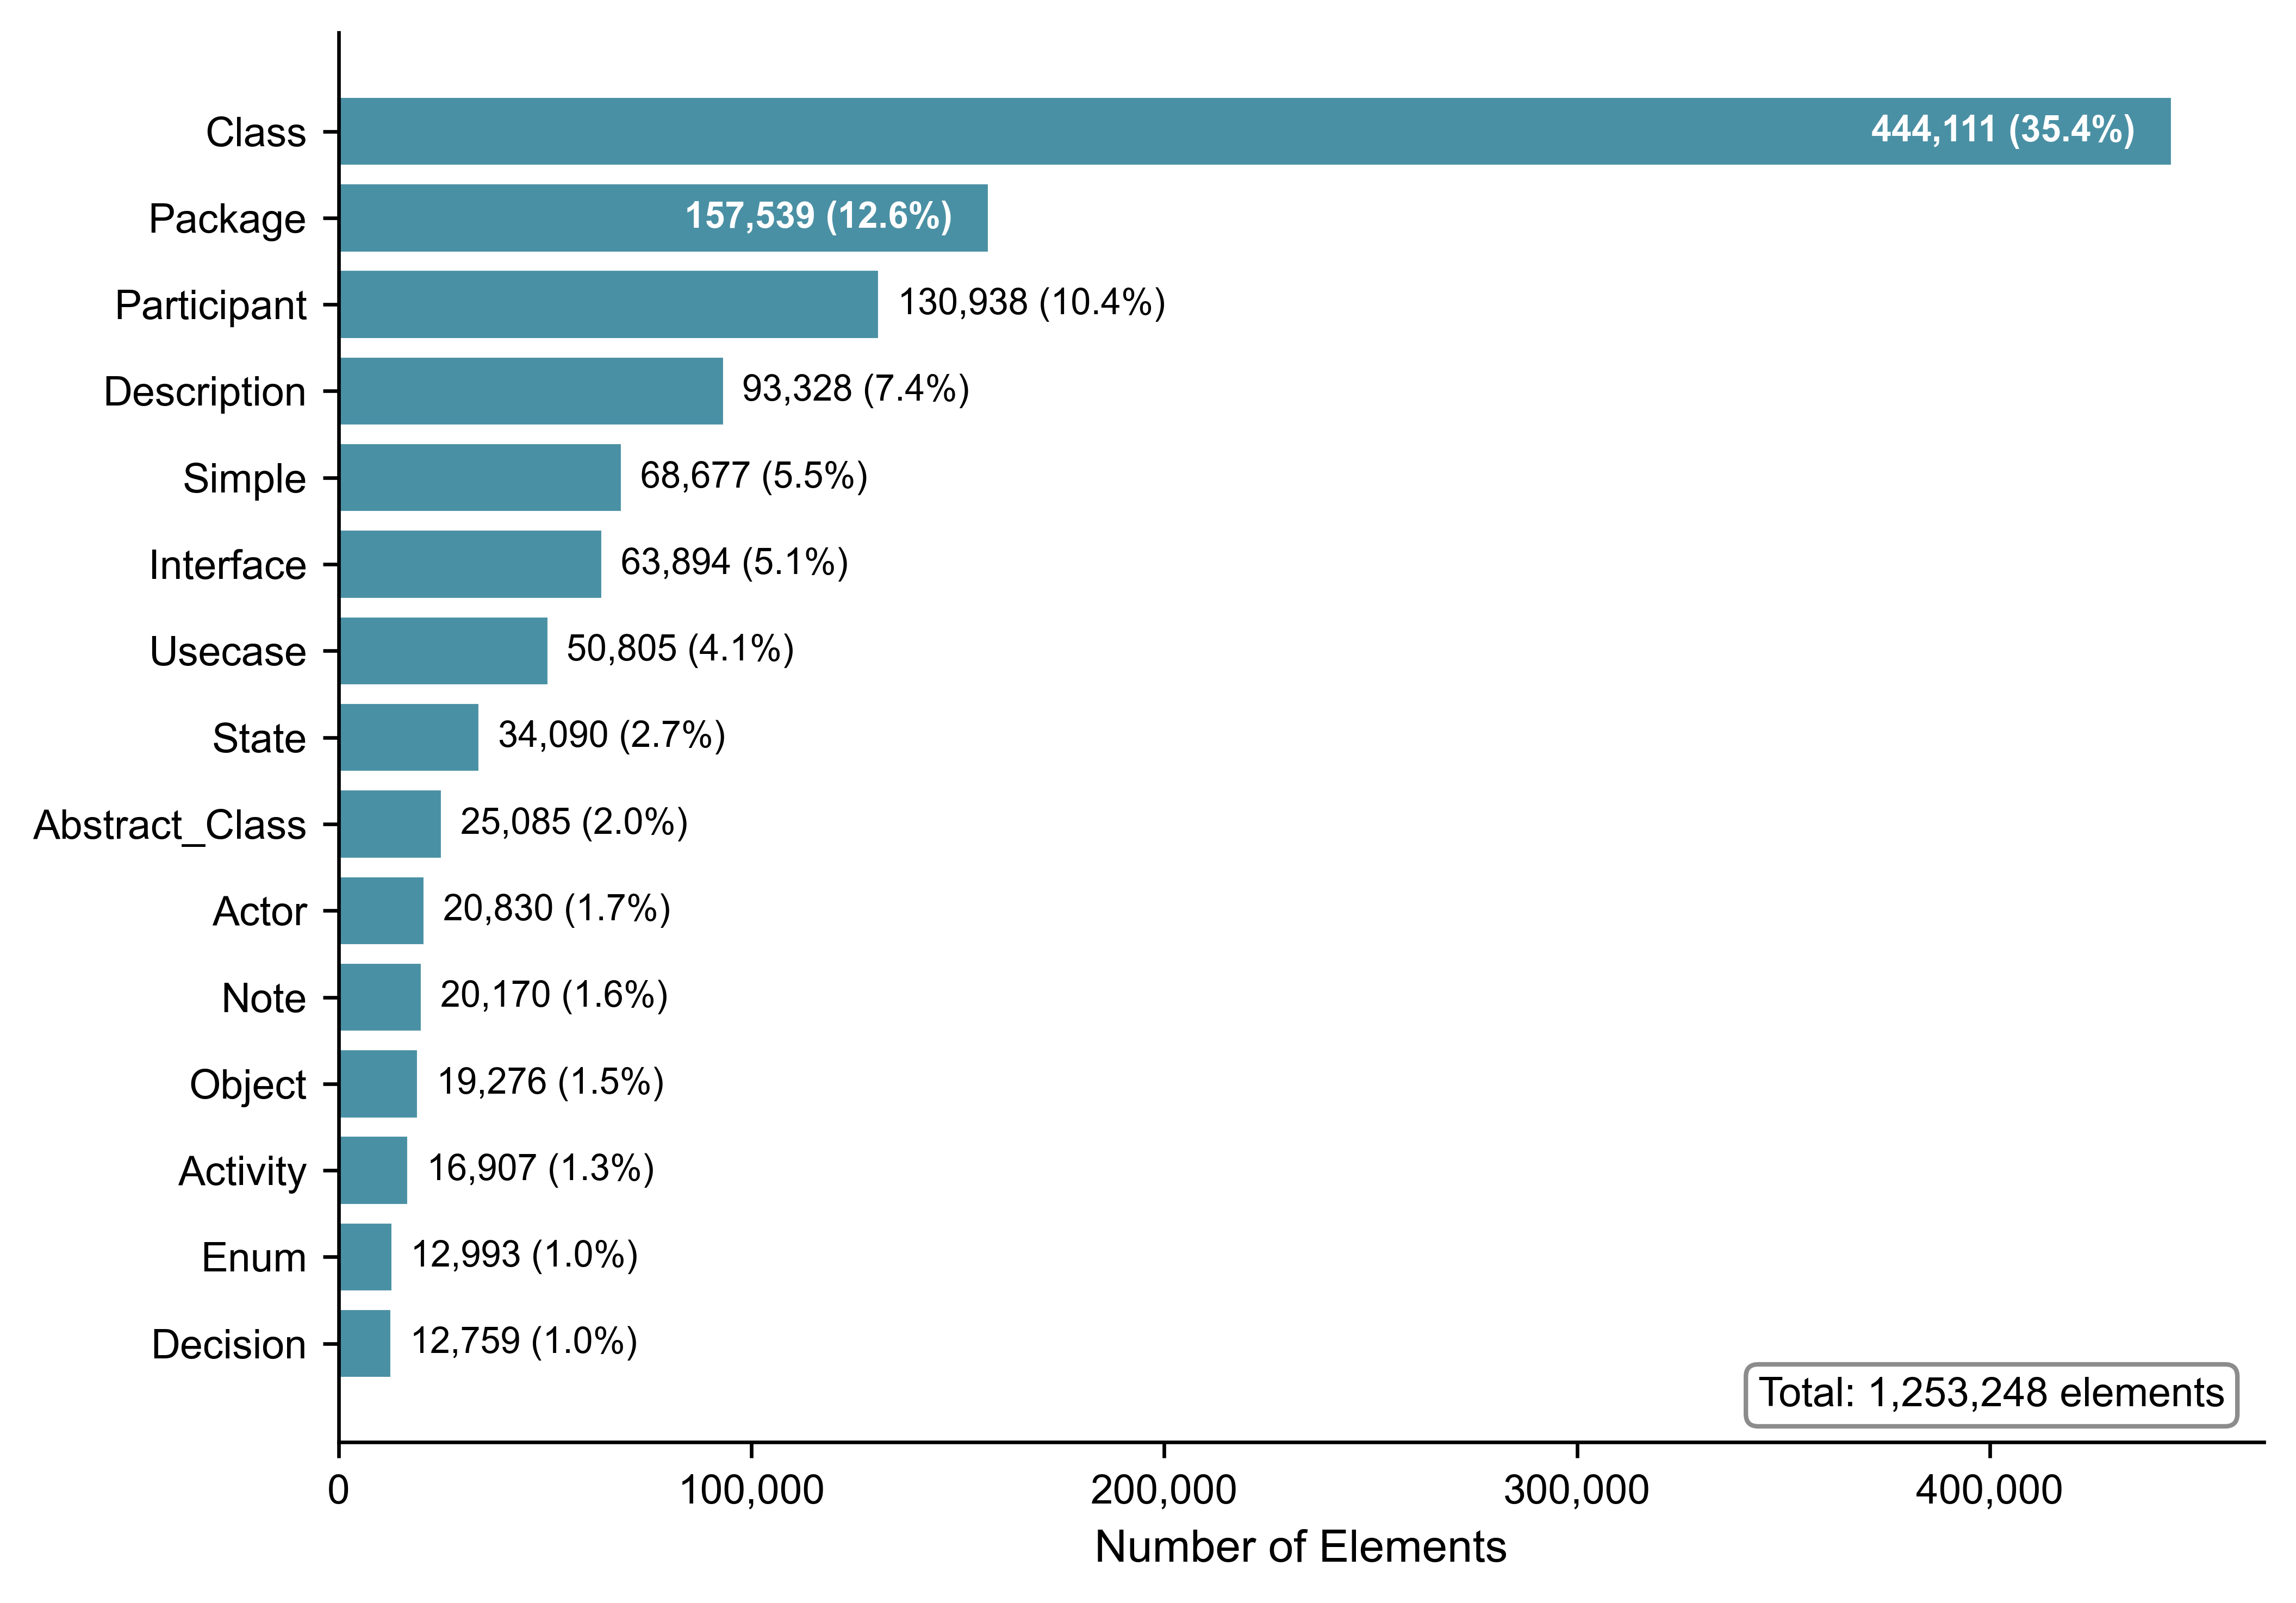
\includegraphics[width=\textwidth]{figures/fig3_element_types.png}
\caption{Top 15 element types across all diagrams.\label{fig:element-types}}
\end{figure}

\begin{figure}[H]
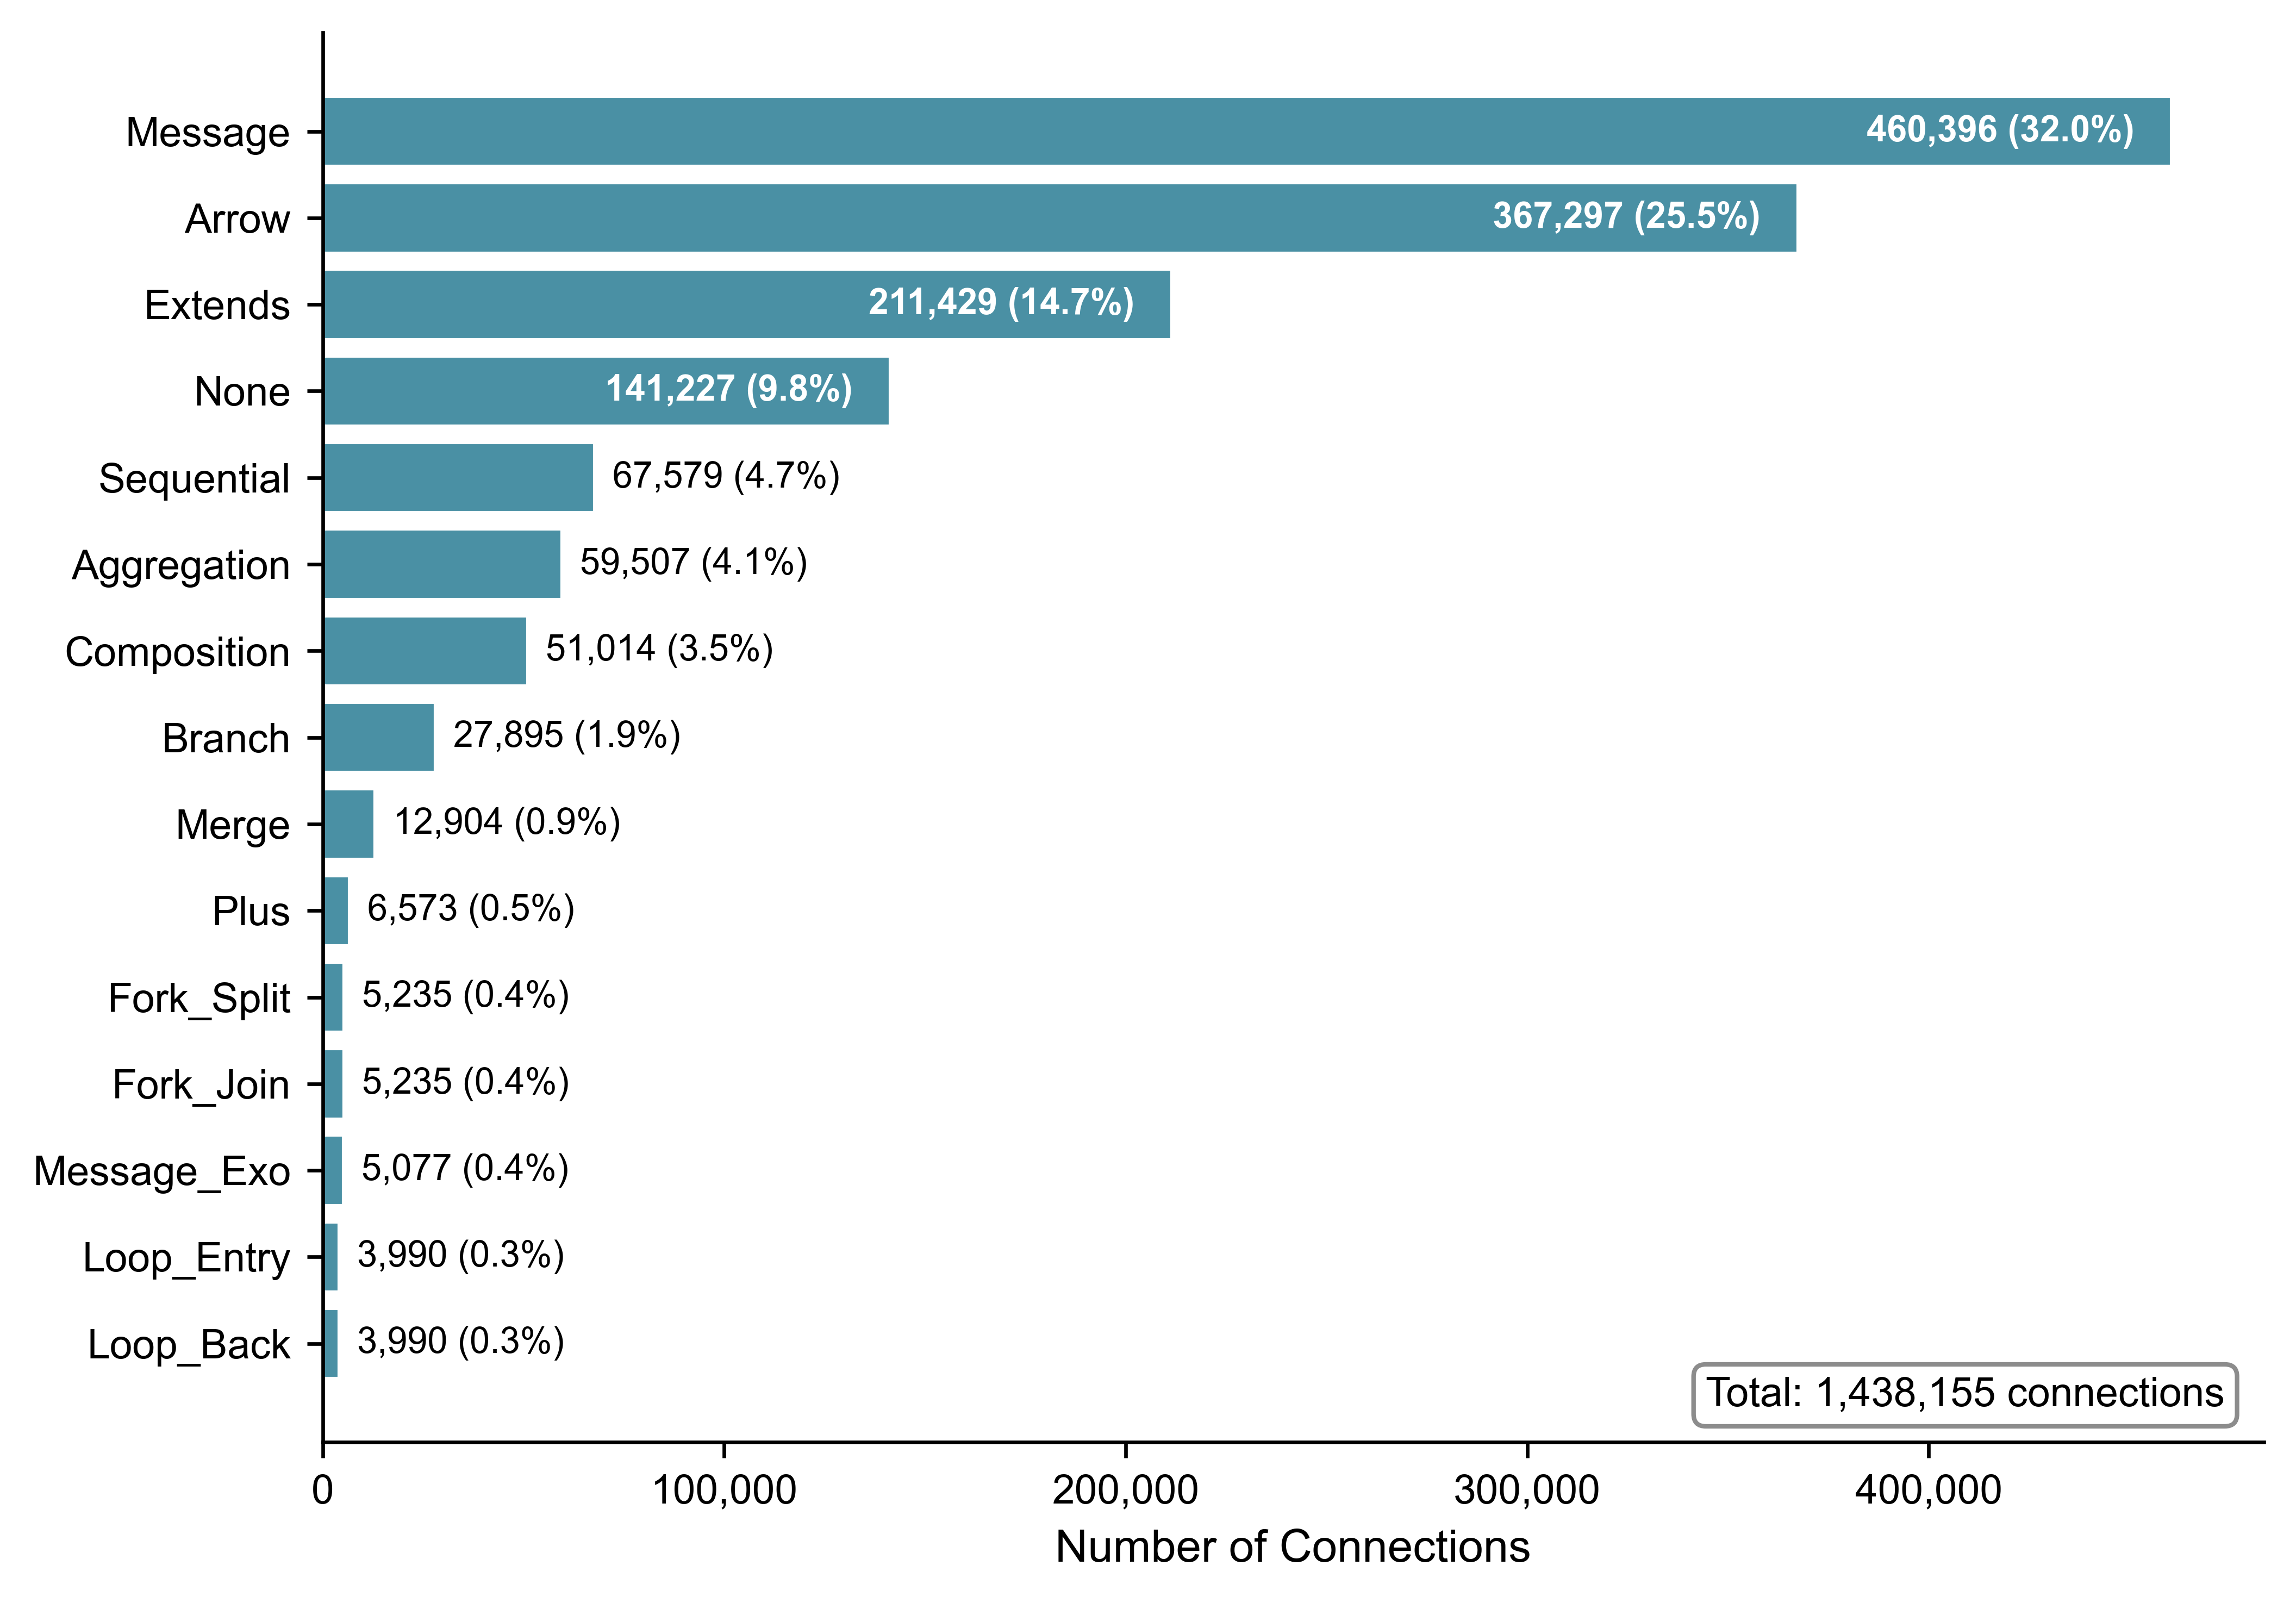
\includegraphics[width=\textwidth]{figures/fig4_connection_categories.png}
\caption{Top 15 connection types across all diagrams.\label{fig:connection-types}}
\end{figure}

\subsection{Metadata Schema}
\label{sec:metadata-schema}

The dataset metadata is stored in a single JSON file with three top-level keys. \texttt{metadata} records pipeline parameters (model identifier, timestamp, file counts). \texttt{statistics} contains pre-computed aggregate analytics---type distributions, element and connection statistics, line count distributions---so that users need not recompute these from individual records. \texttt{classifications} contains one entry per diagram, keyed by filename (e.g., \texttt{"5f95f42b...e89e.puml"}). Table~\ref{tab:metadata-fields} describes the per-diagram fields.

The \texttt{repository} field provides a WoC project identifier in \texttt{\{username\}\_\{reponame\}} format, from which the GitHub URL can be constructed as \url{https://github.com/{username}/{reponame}}. For 1,424 diagrams (1.0\%), the WoC blob-to-project mapping did not contain an entry; these have \texttt{repository} set to \texttt{null}. The diagrams are retained as they are valid UML content---the missing attribution reflects incomplete coverage of the WoC basemap, not a data quality issue.

\begin{table}[H]
\caption{Per-diagram fields in the \texttt{classifications} object.\label{tab:metadata-fields}}
\begin{tabularx}{\textwidth}{lcL}
\toprule
\textbf{Field} & \textbf{Type} & \textbf{Description} \\
\midrule
\texttt{blob\_id}           & string      & SHA-1 content hash (unique identifier) \\
\texttt{original\_path}     & string      & File path within the source repository \\
\texttt{repository}         & string/null & WoC project identifier (\texttt{user\_repo} format); null if unmapped \\
\texttt{primary\_type}      & string      & Diagram type: class, sequence, activity, state, component, usecase, deployment, object, or timing \\
\texttt{secondary\_types}   & array       & Additional types for hybrid diagrams; empty for most entries \\
\texttt{reasoning}          & string      & LLM classification rationale \\
\texttt{content\_lines}     & integer     & Non-blank, non-comment line count \\
\texttt{elements}           & object      & Element counts keyed by type \\
\texttt{elements\_total}    & integer     & Total element count \\
\texttt{connections}        & object      & Connection counts keyed by type \\
\texttt{connections\_total} & integer     & Total connection count \\
\texttt{extraction\_error}  & string/null & Parser error code; null on success \\
\bottomrule
\end{tabularx}
\end{table}

\noindent The following example shows a complete entry for a class diagram with five classes organized in a package, connected by inheritance and composition relationships:

\begin{verbatim}
"473cd312a62f37f459f4a765aa46fb2443ec779d.puml": {
  "blob_id": "473cd312a62f37f459f4a765aa46fb2443ec779d",
  "original_path": "/uml/TodoListClasses.puml",
  "repository": "16smerkel_merkel-cop3330-assignment4",
  "primary_type": "class",
  "secondary_types": [],
  "reasoning": "This is a class diagram defining
    type structures with attributes and ...",
  "content_lines": 38,
  "elements": {"class": 5, "package": 1},
  "elements_total": 6,
  "connections": {"extends": 1, "none": 1,
                  "composition": 2},
  "connections_total": 4,
  "extraction_error": null
}
\end{verbatim}

\noindent Element and connection type labels (e.g., \texttt{none} for an undecorated association line) are derived from PlantUML's internal parser data model; Section~\ref{sec:element-extraction} describes the label semantics in detail.

\subsection{Limitations}
\label{sec:limitations}

The dataset is derived from WoC Version~V, collected in March--May 2023, and does not capture diagrams created or modified after that date. The extraction pipeline identifies PlantUML files solely by six file extensions (\texttt{.puml}, \texttt{.pu}, \texttt{.plantuml}, \texttt{.wsd}, \texttt{.iuml}, \texttt{.uml}); diagrams embedded within Markdown, AsciiDoc, or build tool configurations are not captured. Deduplication relies on SHA-1 blob hashing, which identifies only exact byte-for-byte copies; near-duplicate diagrams differing by minor edits are treated as distinct entries. All diagrams were compiled using PlantUML version 1.2025.9; other versions may produce different compilation outcomes or accept syntax that this version rejects. Finally, 347 diagrams (0.2\%) have empty element and connection fields due to parser extraction failures, predominantly timing diagrams (178) and multi-page diagrams using the \texttt{newpage} keyword (167).


%%%%%%%%%%%%%%%%%%%%%%%%%%%%%%%%%%%%%%%%%%
\section{Methods}
\label{sec:methods}

The dataset was constructed through a three-phase pipeline (Figure~\ref{fig:pipeline}).

In Phase~1 (\emph{Data Extraction}), PlantUML files are identified by extension in the WoC infrastructure, deduplicated by content hash, and validated for well-formed PlantUML markers, yielding 202,106 unique diagrams from an initial 367,550 candidates.

In Phase~2 (\emph{Compilation}), multi-diagram files are split into individual units, tag syntax is normalized to ensure correct compilation, and source files are compiled with PlantUML to produce rendered PNG images, reducing the set to 163,946 successfully compiled diagrams.

In Phase~3 (\emph{Classification and Analysis}), an LLM-based classifier assigns each diagram to one of nine standard UML types, non-UML content is filtered out, and per-diagram structural element and connection counts are extracted using a parser-based tool, producing the final dataset of 143,427 UML diagrams.

The following subsections describe each stage in detail.

\begin{figure}[H]
\centering
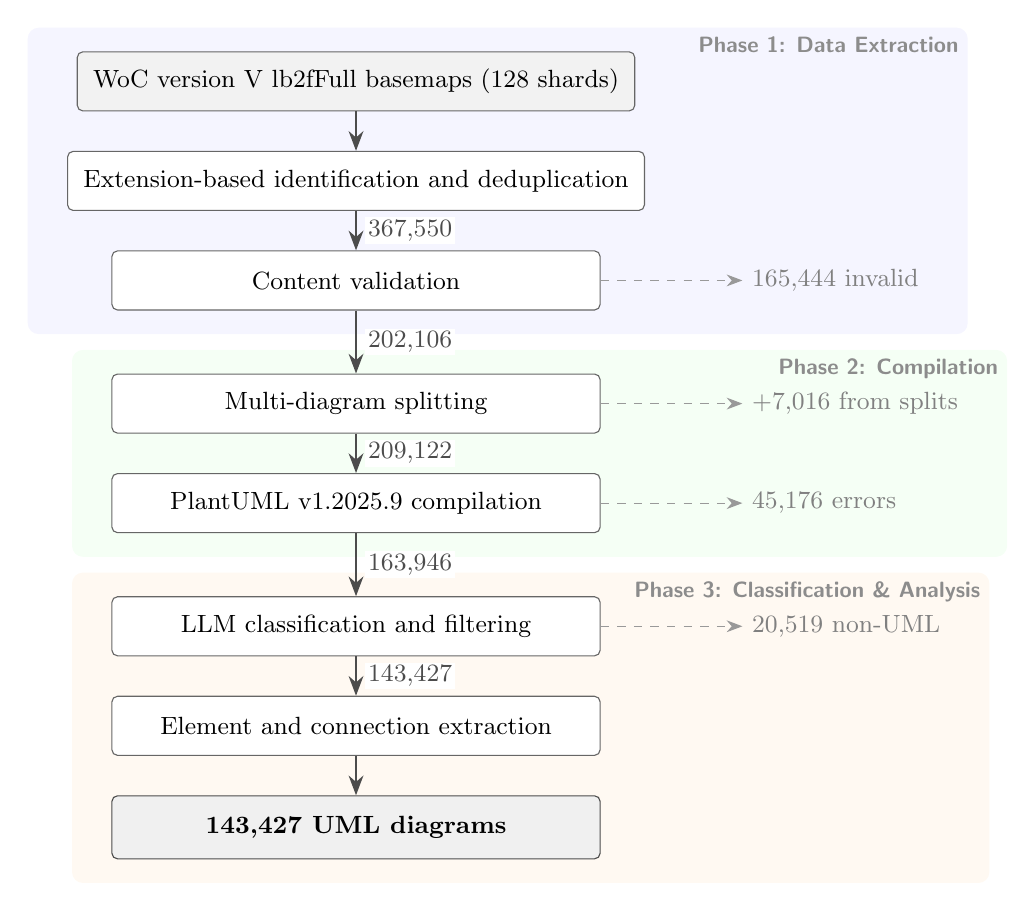
\begin{tikzpicture}[
  node distance=5mm,
  procbox/.style={rectangle, draw=black!60, rounded corners=2pt,
    fill=white, minimum width=62mm, minimum height=7.5mm,
    align=center, font=\small, inner sep=2mm},
  result/.style={rectangle, draw=black!70, rounded corners=2pt,
    fill=black!6, minimum width=62mm, minimum height=8mm,
    align=center, font=\small\bfseries, inner sep=2mm},
  cnt/.style={font=\small, midway, right=3pt, fill=white, inner sep=1pt},
  excl/.style={font=\small, text=black!50},
  arr/.style={-{Stealth[length=2.5mm]}, thick, black!70},
  exarr/.style={-{Stealth[length=2mm]}, thin, dashed, black!40},
  phlbl/.style={font=\footnotesize\bfseries\sffamily, text=black!45, anchor=north east},
]

% Phase 1
\node[procbox, fill=gray!10] (src) {WoC version~V lb2fFull basemaps (128 shards)};
\node[procbox, below=of src] (grep) {Extension-based identification and deduplication};
\node[procbox, below=of grep] (valid) {Content validation};

% Phase 2
\node[procbox, below=8mm of valid] (split) {Multi-diagram splitting};
\node[procbox, below=of split] (compile) {PlantUML v1.2025.9 compilation};

% Phase 3
\node[procbox, below=8mm of compile] (classify) {LLM classification and filtering};
\node[procbox, below=of classify] (extract) {Element and connection extraction};

% Result
\node[result, below=of extract] (final) {143,427 UML diagrams};

% Main flow arrows with counts
\draw[arr] (src) -- (grep);
\draw[arr] (grep) -- node[cnt] {367,550} (valid);
\draw[arr] (valid) -- node[cnt] {202,106} (split);
\draw[arr] (split) -- node[cnt] {209,122} (compile);
\draw[arr] (compile) -- node[cnt] {163,946} (classify);
\draw[arr] (classify) -- node[cnt] {143,427} (extract);
\draw[arr] (extract) -- (final);

% Exclusion branches
\node[excl, right=18mm of valid] (e1) {165,444 invalid};
\draw[exarr] (valid.east) -- (e1.west);

\node[excl, right=18mm of split] (e0) {+7,016 from splits};
\draw[exarr] (split.east) -- (e0.west);

\node[excl, right=18mm of compile] (e2) {45,176 errors};
\draw[exarr] (compile.east) -- (e2.west);

\node[excl, right=18mm of classify] (e3) {20,519 non-UML};
\draw[exarr] (classify.east) -- (e3.west);

% Phase backgrounds
\begin{scope}[on background layer]
  \node[rectangle, rounded corners=4pt, fill=blue!4,
    inner xsep=5mm, inner ysep=3mm,
    fit=(src)(grep)(valid)(e1)] (p1) {};
  \node[rectangle, rounded corners=4pt, fill=green!4,
    inner xsep=5mm, inner ysep=3mm,
    fit=(split)(compile)(e0)(e2)] (p2) {};
  \node[rectangle, rounded corners=4pt, fill=orange!5,
    inner xsep=5mm, inner ysep=3mm,
    fit=(classify)(extract)(final)(e3)] (p3) {};
\end{scope}

% Phase labels
\node[phlbl] at (p1.north east) {Phase~1: Data Extraction};
\node[phlbl] at (p2.north east) {Phase~2: Compilation};
\node[phlbl] at (p3.north east) {Phase~3: Classification \& Analysis};

\end{tikzpicture}
\caption{Overview of the data extraction and processing pipeline. Counts on arrows indicate the number of items flowing between steps; dashed arrows show items excluded at each filtering stage.\label{fig:pipeline}}
\end{figure}

\subsection{Data Source}
\label{sec:data-source}

The dataset was constructed using WoC~\cite{ma2021world}, a comprehensive collection of open-source repositories maintained by the University of Tennessee, Knoxville. WoC releases are designated by sequential letters; we used version~V, whose snapshot was built from updates and new repositories identified during March~1--30, 2023, with git objects retrieved by mid-May~2023. This version indexes over 209~million repositories and 16.2~billion blobs (unique file contents).

The primary data structure used for file identification was the \texttt{lb2fFull} basemap, which consists of 128 sharded files mapping blob identifiers (SHA-1 hashes) to their corresponding file paths in the format \texttt{blob\_id;file\_path}. Since WoC uses content-addressable storage, each blob identifier uniquely represents a distinct file content regardless of how many repositories contain copies of that file.

\subsection{File Identification and Content Validation}
\label{sec:identification-validation}

To identify candidate PlantUML files, we performed a case-insensitive regular expression search across all 128~\texttt{lb2fFull} basemap shards, matching file paths that end with one of six PlantUML-associated extensions: \texttt{.puml}, \texttt{.pu}, \texttt{.plantuml}, \texttt{.wsd}, \texttt{.iuml}, and \texttt{.uml}. The search yielded 504,451~file entries in total. Because WoC's content-addressable storage allows the same blob to appear under multiple file paths across different repositories and branches, we deduplicated the results by blob identifier, retaining a single arbitrarily selected path per unique SHA-1 hash (the lexicographically first entry produced by the Unix \texttt{sort~-u} command). After deduplication, 367,550~unique blobs remained as candidates.

For each candidate blob, we retrieved the actual file content from WoC storage and checked for the presence of PlantUML boundary markers. A file was accepted only if it contained both an \texttt{@startuml} and an \texttt{@enduml} marker in a case-insensitive substring match. Of the 367,550~unique blobs, 202,106 (55.0\%) passed this validation, 163,802 (44.6\%) lacked the required markers, and 1,642 (0.4\%) could not be retrieved from WoC storage.

The six targeted extensions differ substantially in their specificity as indicators of PlantUML content, as shown in Table~\ref{tab:extension-validation}. The dedicated extensions \texttt{.plantuml} and \texttt{.puml} exhibit the highest validation rates (96.7\% and 85.1\%, respectively), confirming that they are reliable markers of PlantUML source files. The \texttt{.pu} and \texttt{.wsd} extensions also show moderate-to-high validity (80.2\% and 63.1\%). In contrast, the \texttt{.iuml} extension achieves only 52.4\% validity because it is conventionally used for PlantUML include fragments that define reusable components such as macros or styling directives and often lack the required structural markers. The generic \texttt{.uml} extension has the lowest validation rate at 5.4\%, as the vast majority of \texttt{.uml} files contain alternative UML representations such as XMI or Eclipse UML metadata rather than PlantUML notation. Despite this low yield, including the \texttt{.uml} extension contributed 7,186~valid blobs to the dataset, justifying its retention in the extraction pipeline.

This extension-based approach was chosen because a content-based alternative---scanning all 16.2~billion blobs in WoC for \texttt{@startuml} markers---would be computationally prohibitive. The six targeted extensions are consistent with those identified by Romeo et al.~\cite{romeo2025uml} as the most prevalent UML formats in well-established open-source projects. However, this approach does not capture PlantUML content stored in files with non-standard extensions or embedded within other document formats such as Markdown or AsciiDoc; this limitation is noted in Section~\ref{sec:limitations}.

\begin{table}[H]
\caption{PlantUML content validation rate by file extension.\label{tab:extension-validation}}
\begin{tabularx}{\textwidth}{lCCCC}
\toprule
\textbf{Extension} & \textbf{Valid} & \textbf{Invalid} & \textbf{Total} & \textbf{Valid Rate (\%)} \\
\midrule
\texttt{.plantuml} & 21,980  & 746     & 22,726  & 96.7 \\
\texttt{.puml}     & 146,851 & 25,766  & 172,617 & 85.1 \\
\texttt{.pu}       & 10,004  & 2,472   & 12,476  & 80.2 \\
\texttt{.wsd}      & 14,862  & 8,709   & 23,571  & 63.1 \\
\texttt{.iuml}     & 1,223   & 1,109   & 2,332   & 52.4 \\
\texttt{.uml}      & 7,186   & 124,998 & 132,184 & 5.4 \\
\bottomrule
\end{tabularx}
\noindent{\footnotesize{Excludes 2 blobs with no recognized extension (both invalid) and 1,642 blobs that could not be retrieved from WoC storage.}}
\end{table}

\subsection{Preprocessing and Normalization}
\label{sec:preprocessing}

Before compilation, two preprocessing steps improve the correspondence between source files and individual diagrams and preserve the blob-ID-based naming convention described in Section~\ref{sec:file-naming}.

PlantUML allows multiple diagrams to be defined within a single file using successive \texttt{@startuml...@enduml} blocks. Of the 202,106~validated files, 1,842 (0.9\%) contained two or more diagram blocks. A splitting algorithm detects all \texttt{@start\textit{type}...@end\textit{type}} pairs (including non-UML types such as \texttt{@startditaa} and \texttt{@startsalt}) using case-insensitive regular expression matching. Each block is extracted into a separate file named \texttt{\{blob\_id\}\_01.puml}, \texttt{\{blob\_id\}\_02.puml}, etc., with the pipeline-injected metadata header copied to every resulting file to preserve provenance. Single-diagram files are left unchanged. This process increased the total file count from 202,106 to 209,122, yielding 7,016~additional diagram files from the multi-diagram sources.

Following the split, a tag normalization step addresses two issues that would otherwise interfere with compilation. PlantUML's \texttt{@startuml} directive accepts an optional name argument---via braces (\texttt{@startuml\{name\}}), parentheses, brackets, or a space-separated token---that overrides the output filename. Because the dataset uses blob IDs as canonical filenames, retaining these custom names would produce PNG files whose names no longer match their source files, breaking the metadata linkage. Additionally, commented-out diagram directives (e.g., \texttt{'\,@startuml}) can cause the compiler to generate spurious output images. To address both issues, we applied two in-place normalizations: (1)~stripping all custom name arguments from \texttt{@start\textit{type}} directives, and (2)~removing commented-out \texttt{@start}/\texttt{@end} lines. Of the 209,122~files, 35,612 (17.0\%) required at least one of these modifications; the remaining files were left unchanged. The total file count was unaffected by this step.

\subsection{Image Generation}
\label{sec:image-generation}

The 209,122 preprocessed \texttt{.puml} files were compiled into PNG images using PlantUML version~1.2025.9. The compiler was invoked with the \texttt{-{}-no-error-image} flag, which suppresses the generation of placeholder error images for files that fail compilation; without this flag, PlantUML produces a red error image for every failed file, which would conflate valid and invalid outputs. By disabling error images, the presence of a PNG file serves as a direct indicator of successful compilation.

Of the 209,122 input files, 163,946 (78.4\%) compiled successfully and 45,176 (21.6\%) produced compilation errors. The compilation process generated 165,177~PNG images in total---slightly more than the 163,946 successfully compiled files because PlantUML's \texttt{newpage} keyword splits a single diagram into multiple output pages, each rendered as a separate PNG file following the naming convention described in Section~\ref{sec:file-naming}.

Beyond rendering, the compilation step functions as a syntactic validation layer: a file that passes compilation is confirmed to be well-formed PlantUML that the tool can parse and render, whereas compilation failure indicates syntax errors, unresolvable includes, or other structural issues. Only the 163,946 successfully compiled diagrams proceed to the classification stage (Section~\ref{sec:classification}).

\subsection{Diagram Type Classification}
\label{sec:classification}

PlantUML uses a single \texttt{@startuml} keyword for all nine standard UML diagram types, determining the specific type at parse time through an ordered factory chain that matches content against type-specific syntax rules. Because the keyword alone cannot distinguish a class diagram from a sequence or state diagram, an automated classifier is required. We employed Claude Haiku~4.5 (model identifier \texttt{claude-haiku-4-5-20251001}) via the Anthropic Message Batches API to classify all 163,946 compiled diagrams. Each diagram's preprocessed PlantUML source was submitted with a structured prompt instructing the model to classify by semantic meaning---content and intent---rather than syntax alone.

Before classification, each diagram undergoes a lightweight preprocessing pipeline that reduces token consumption while preserving signals relevant to type identification. The pipeline removes pipeline-injected metadata headers (blob ID, original path, and source comments), sprite definitions (both hex/raster and SVG inline sprites), preprocessor procedure and function bodies, hyperlink syntax, and documentation blocks (headers, footers, legends, and captions). Multi-line notes are collapsed to single-line markers, and excessive blank lines are reduced. Crucially, the pipeline preserves elements that carry strong type signals: human-authored comments, which often describe diagram purpose; styling directives (\texttt{skinparam}, \texttt{hide}, \texttt{show}); standard library includes (\texttt{!include}); macro definitions (\texttt{!define}), which frequently map aliases to diagram element types; and title lines. Files exceeding 5000~words were truncated to 4000~words to stay within the model's effective context window while retaining the structurally informative beginning of the file.

For each diagram, the classifier produces three fields: \texttt{primary\_type}, assigned as one of nine standard UML types (class, sequence, activity, state, component, usecase, deployment, object, or timing) or \texttt{non-uml}; \texttt{secondary\_types}, populated only when a diagram genuinely combines elements from multiple UML diagram types, which occurs in 983~diagrams (0.7\% of the final dataset); and \texttt{reasoning}, a one-sentence rationale for the classification decision.

Of the 163,946 classified diagrams, 20,434 (12.5\%) were assigned the \texttt{non-uml} label. This category comprises predominantly sprite and icon library definitions---files that define reusable graphical sprites using PlantUML's sprite directive and \texttt{!define} macros---as well as PlantUML-specific non-UML formats (\texttt{@startmindmap}, \texttt{@startgantt}, \texttt{@startwbs}, \texttt{@startjson}, \texttt{@startsalt}, \texttt{@startditaa}, \texttt{@startnwdiag}, \texttt{@startdot}), ERD and database schemas using crow's foot notation, and empty or unrecognizable files. Since these do not constitute standard UML diagrams, all 20,434 entries were removed, reducing the dataset to 143,512~diagrams. Two additional filtering steps further refined the dataset. First, 84~diagrams were identified as Graphviz DOT passthrough---raw \texttt{digraph}/\texttt{graph} syntax wrapped in \texttt{@startuml} that PlantUML forwards to Graphviz without constructing a UML model. These were detected by the parser-based extraction tool described in Section~\ref{sec:element-extraction}, which reports the error code \texttt{unsupported\_type:PSystemDot} for such files; although the LLM had classified these as UML types, the parser's structural analysis revealed they are not UML diagrams. Second, one diagram with zero content lines was removed. The resulting dataset contains 143,427 UML diagrams across 9~standard types. The classification is validated in Section~\ref{sec:validation}.

\subsection{Element and Connection Extraction}
\label{sec:element-extraction}

To quantify the structural complexity of each diagram, we developed a parser-based extraction tool that counts typed elements (nodes) and connections (edges). Rather than using regular expressions---which would require reimplementing PlantUML's handling of multiple syntactic forms for the same construct, alias resolution, namespace qualification, macro expansion, and file includes---the tool reuses PlantUML's own parsing pipeline. This ensures that element and connection counts reflect the same interpretation of the source that the compiler applies when rendering.

The tool is implemented as a Java class (\texttt{DiagramStatsExtractor}) embedded within the PlantUML source tree (version~1.2025.9)\footnote{Available at \url{https://github.com/vovanrew/plantuml}, archived at \url{https://doi.org/10.5281/zenodo.19288003}.}. For each input file, it invokes PlantUML's full parsing pipeline---preprocessing (macro expansion, \texttt{!include} resolution, conditional compilation), diagram type detection, and type-specific command interpretation---to produce a fully resolved diagram object. The tool then inspects this object to extract per-type element and connection counts. No modifications were made to PlantUML's parsing logic, command definitions, or diagram construction code.

Three extraction strategies are dispatched based on the diagram's internal representation. The \emph{entity-link strategy} handles six diagram types (class, object, component, deployment, use case, and state) that share a common internal representation with separate entity and link collections. Elements are read from the entity collection and typed by their internal label (e.g., \texttt{class}, \texttt{interface}, \texttt{enum}, \texttt{component}, \texttt{state}, \texttt{usecase}, \texttt{package}). Connections are read from the link collection. When a link carries different decorations on each end, the tool classifies it by the more semantically specific one, following a priority order: \texttt{extends}, \texttt{composition}, \texttt{aggregation}, \texttt{arrow}, \texttt{none} (with two rarely occurring UML redefinition types, \texttt{redefines} and \texttt{definedby}, ranked between \texttt{aggregation} and \texttt{arrow}).

The \emph{sequence strategy} handles sequence diagrams. Participants are counted as elements by their declared type (\texttt{participant}, \texttt{actor}, \texttt{boundary}, \texttt{control}, \texttt{entity}, \texttt{database}, \texttt{collections}, \texttt{queue}). Messages are counted as connections: inter-participant messages as \texttt{message} and external messages (directed to or from outside the diagram boundary) as \texttt{message\_exo}. Combined fragments (\texttt{alt}, \texttt{opt}, \texttt{loop}), notes, dividers, and references are not counted, as they represent behavioral annotations rather than graph structure.

The \emph{activity strategy} handles activity diagrams by traversing PlantUML's tree-structured intermediate representation. Nodes are counted as elements with labels derived from PlantUML's internal instruction types (e.g., \texttt{simple} for action nodes, \texttt{decision} for conditional nodes, \texttt{loop}, \texttt{fork}, \texttt{start}, \texttt{stop}). Control flow edges between nodes are counted as connections (\texttt{sequential}, \texttt{branch}, \texttt{merge}, \texttt{loop\_entry}/\texttt{loop\_back}/\texttt{loop\_exit}, \texttt{fork\_split}/\texttt{fork\_join}). These connections represent edges in the abstract control flow graph, not visual arrows in the rendered diagram---compound instructions may share a single visual arrow while having distinct structural edges.

Two characteristics of PlantUML's internal representation affect the resulting counts. First, in entity-link diagrams, PlantUML injects synthetic links into its parsed link collection for rendering purposes---note-attachment links that anchor notes to entities, and layout links generated for internal arrangement. Because these synthetic links carry no distinguishing marker, the extraction tool cannot separate them from user-declared undecorated associations; both appear as \texttt{none} connections. Second, in activity diagrams, the tool unconditionally counts convergence edges for compound instructions (if/switch/fork blocks), even when all branches terminate before reaching the merge point, resulting in a slight connection overcount in such diagrams. Of the 143,427 diagrams in the dataset, 143,080 were successfully processed by the extraction tool; the remaining 347 are reported with an \texttt{extraction\_error} code in the metadata.

\subsection{Validation}
\label{sec:validation}

To assess the accuracy of the automated classification and extraction stages, we performed a manual validation study on a stratified random sample of 270~diagrams---30~per diagram type across all 9~types---selected with a fixed random seed~(42) for reproducibility. A single domain expert (the first author) reviewed each diagram by reading the PlantUML source file. The validation followed a two-layered design. In Layer~1, the reviewer independently determined the diagram type and counted total elements and connections without consulting the tool's output, eliminating confirmation bias on aggregate totals. In Layer~2, the reviewer examined the tool's per-type breakdown against reference tables documenting all 57~element type keys and 28~connection type keys, verifying or correcting individual counts. The validation is source-based rather than visual: the extraction tool operates on PlantUML's parsed intermediate representation, and activity diagram connections represent control flow graph edges that do not have one-to-one visual counterparts, as discussed in Section~\ref{sec:element-extraction}. The complete validation records and reference tables are available in the dataset deposit.

The LLM-based classifier achieved an overall accuracy of 95.9\% (259/270). Four diagram types---class, deployment, state, and use case---achieved 100\% accuracy (30/30 each). Figure~\ref{fig:confusion-matrix} shows the confusion matrix. Two systematic confusion patterns account for 8 of the 11 misclassifications. First, 5 timing diagrams were misclassified as sequence diagrams; all five were sequence diagrams that use the \texttt{!pragma teoz} timing constraint syntax, which introduces temporal ordering semantics but does not change the diagram type. Second, 3 component diagrams were misclassified as class diagrams; in each case, class declarations inside packages led the classifier to assign the class type. The remaining 3 errors are isolated single-instance confusions: one activity diagram classified as state, one object diagram classified as component, and one sequence diagram classified as component.

\begin{figure}[H]
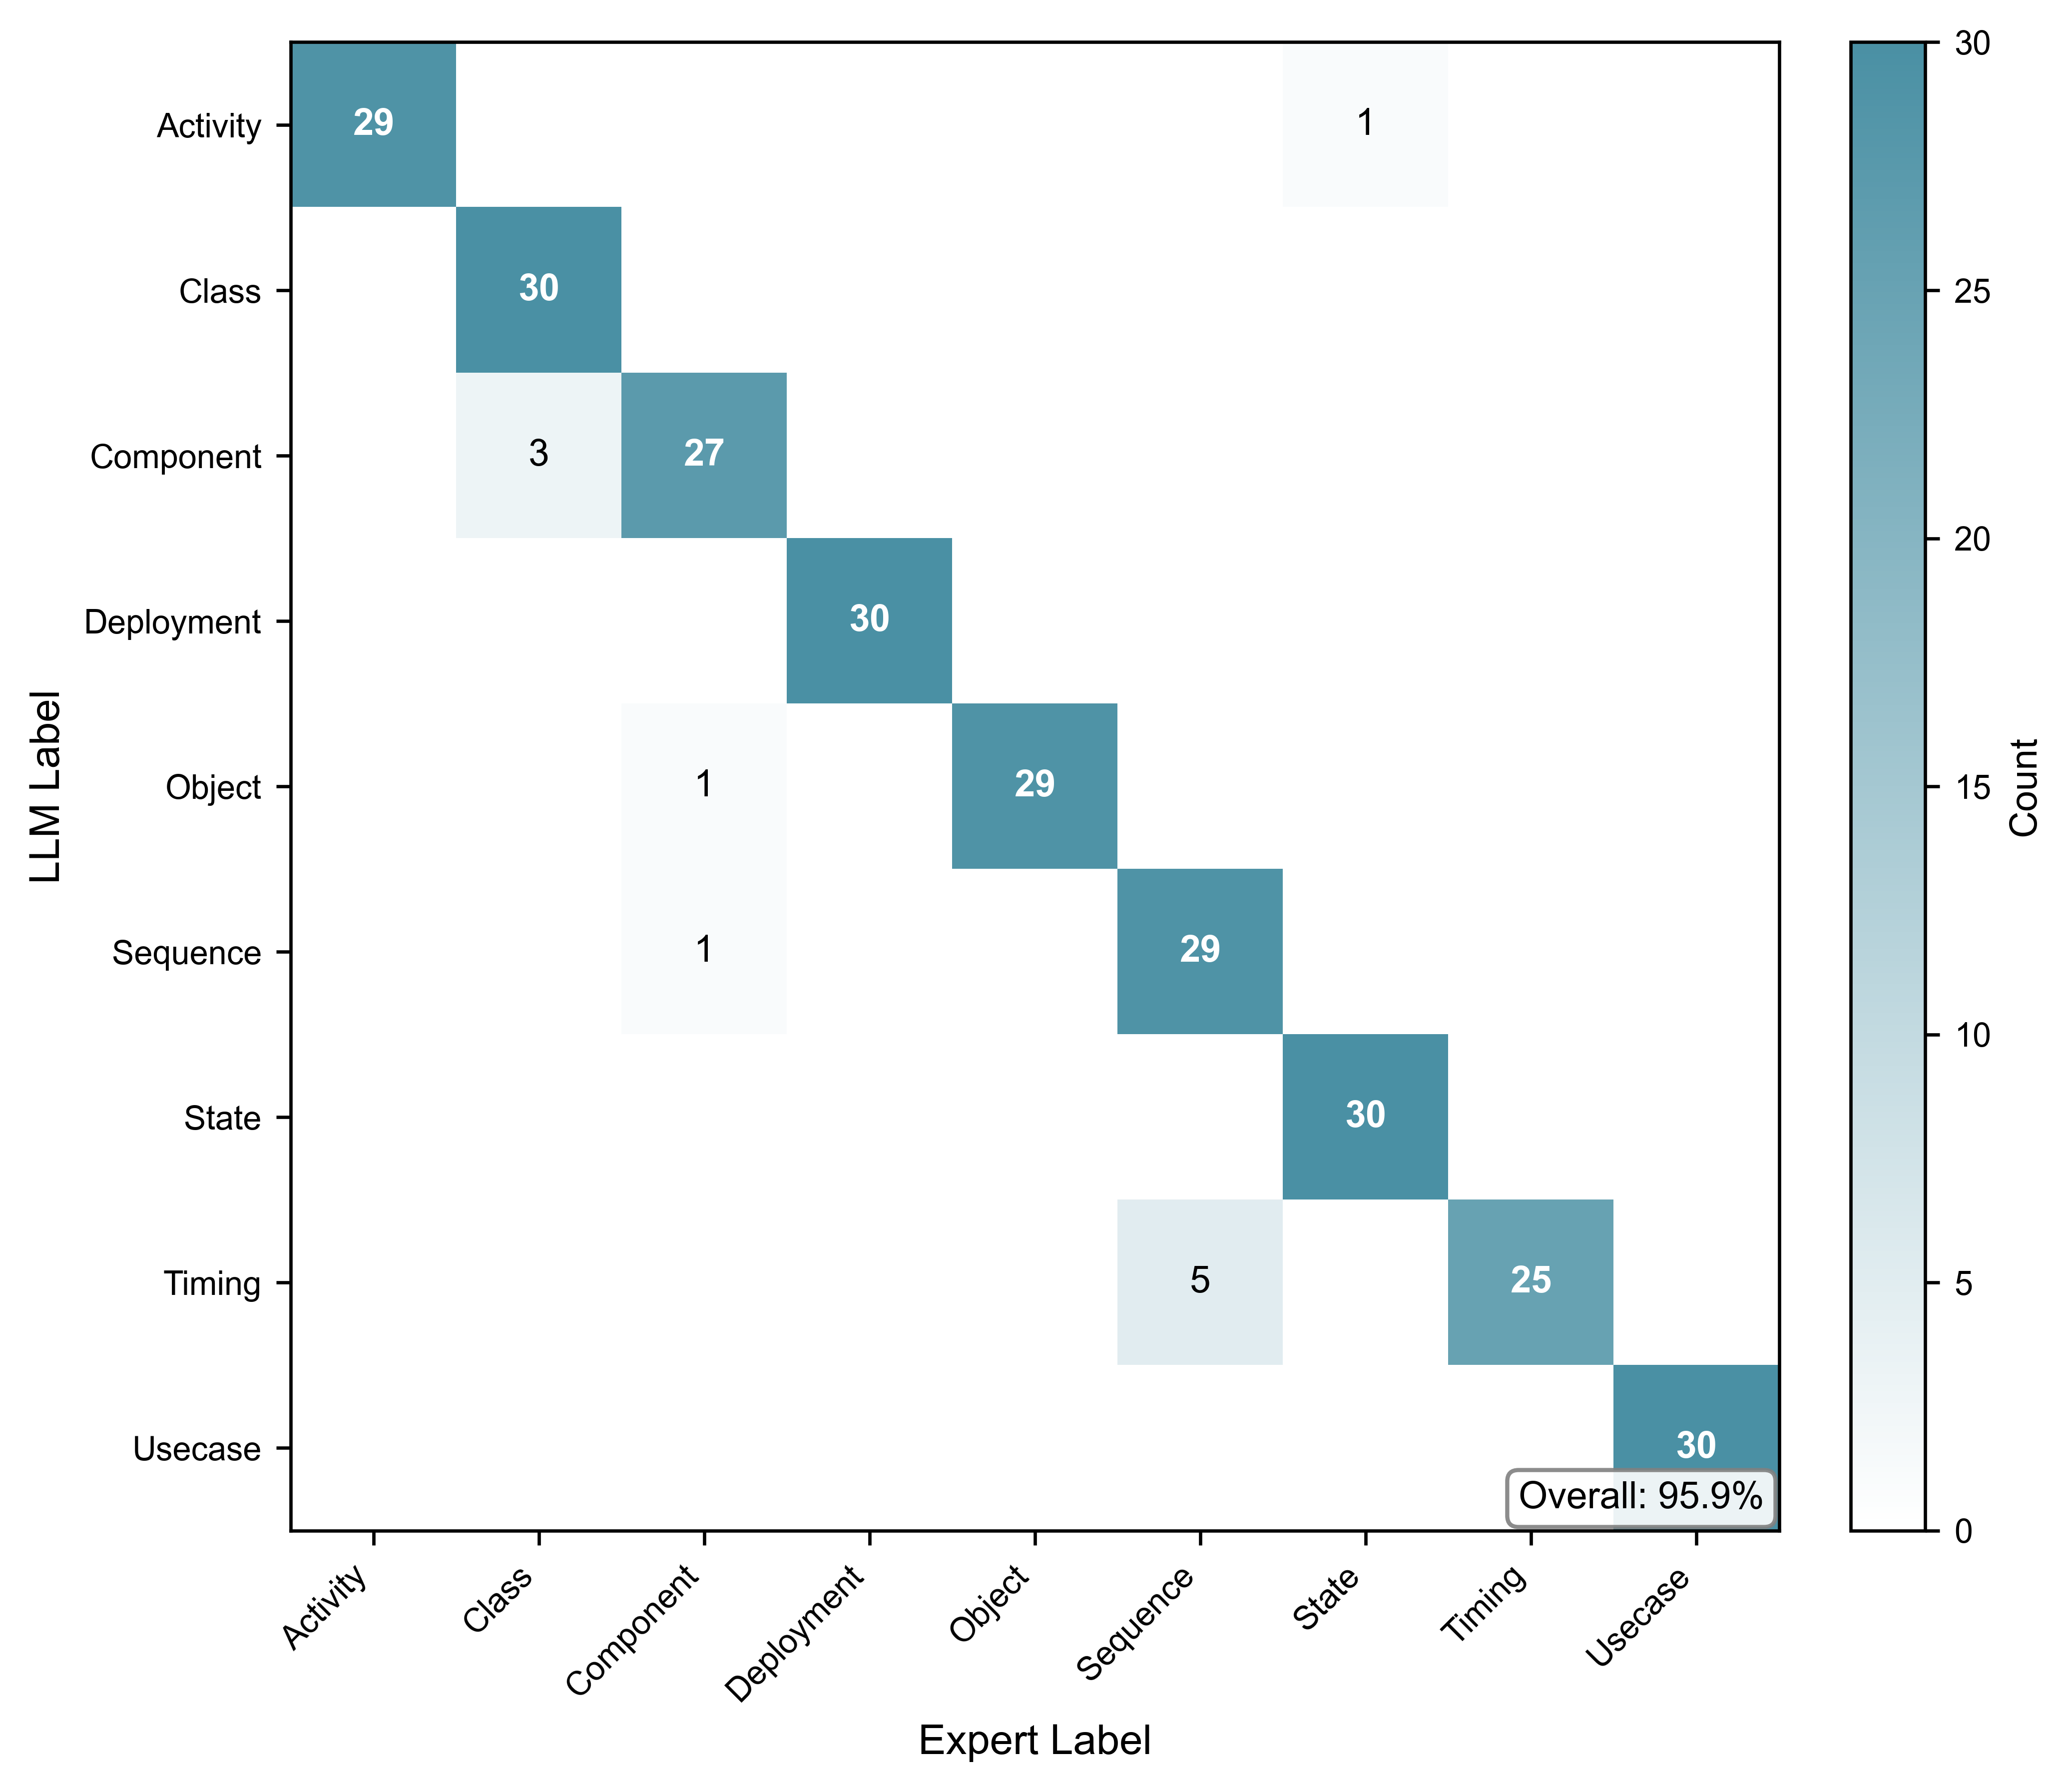
\includegraphics[width=\textwidth]{figures/fig5_confusion_matrix.png}
\caption{Confusion matrix for diagram type classification (270-diagram validation sample, 30~per type). Rows represent the LLM-assigned type; columns represent the expert-assigned type. Off-diagonal entries indicate misclassifications.\label{fig:confusion-matrix}}
\end{figure}

Element and connection extraction accuracy was evaluated on 240~diagrams, excluding the 30~timing diagrams (see below). Element extraction achieved a 99.2\% exact match rate (238/240). Only 2~diagrams exhibited element count mismatches, both complete extraction failures: one caused by the \texttt{newpage} keyword splitting the diagram mid-parse, and one reporting 0~elements and 0~connections.

Connection extraction achieved an 88.3\% exact match rate (212/240). Of the 28~mismatches, 27~were overcounts and 1~was an undercount, with a median overcount of 2~connections among affected diagrams. Two systematic causes account for the vast majority of errors. The first is synthetic links injected by PlantUML into its internal link collection for rendering purposes---primarily note-attachment links and layout arrangement links---which the extraction tool cannot distinguish from user-declared associations, as discussed in Section~\ref{sec:element-extraction}. This affected class diagrams (8/30), use case diagrams (7/30), deployment diagrams (5/30), state diagrams (3/30), and component diagrams (2/30). The second cause is unreachable merge edges in activity diagrams: the tool counts convergence edges for compound instructions (\texttt{if}/\texttt{fork}/\texttt{switch} blocks) even when all branches terminate before reaching the merge point, producing 3~overcounts. Figure~\ref{fig:validation-accuracy} presents the per-type breakdown of element and connection exact match rates.

\begin{figure}[H]
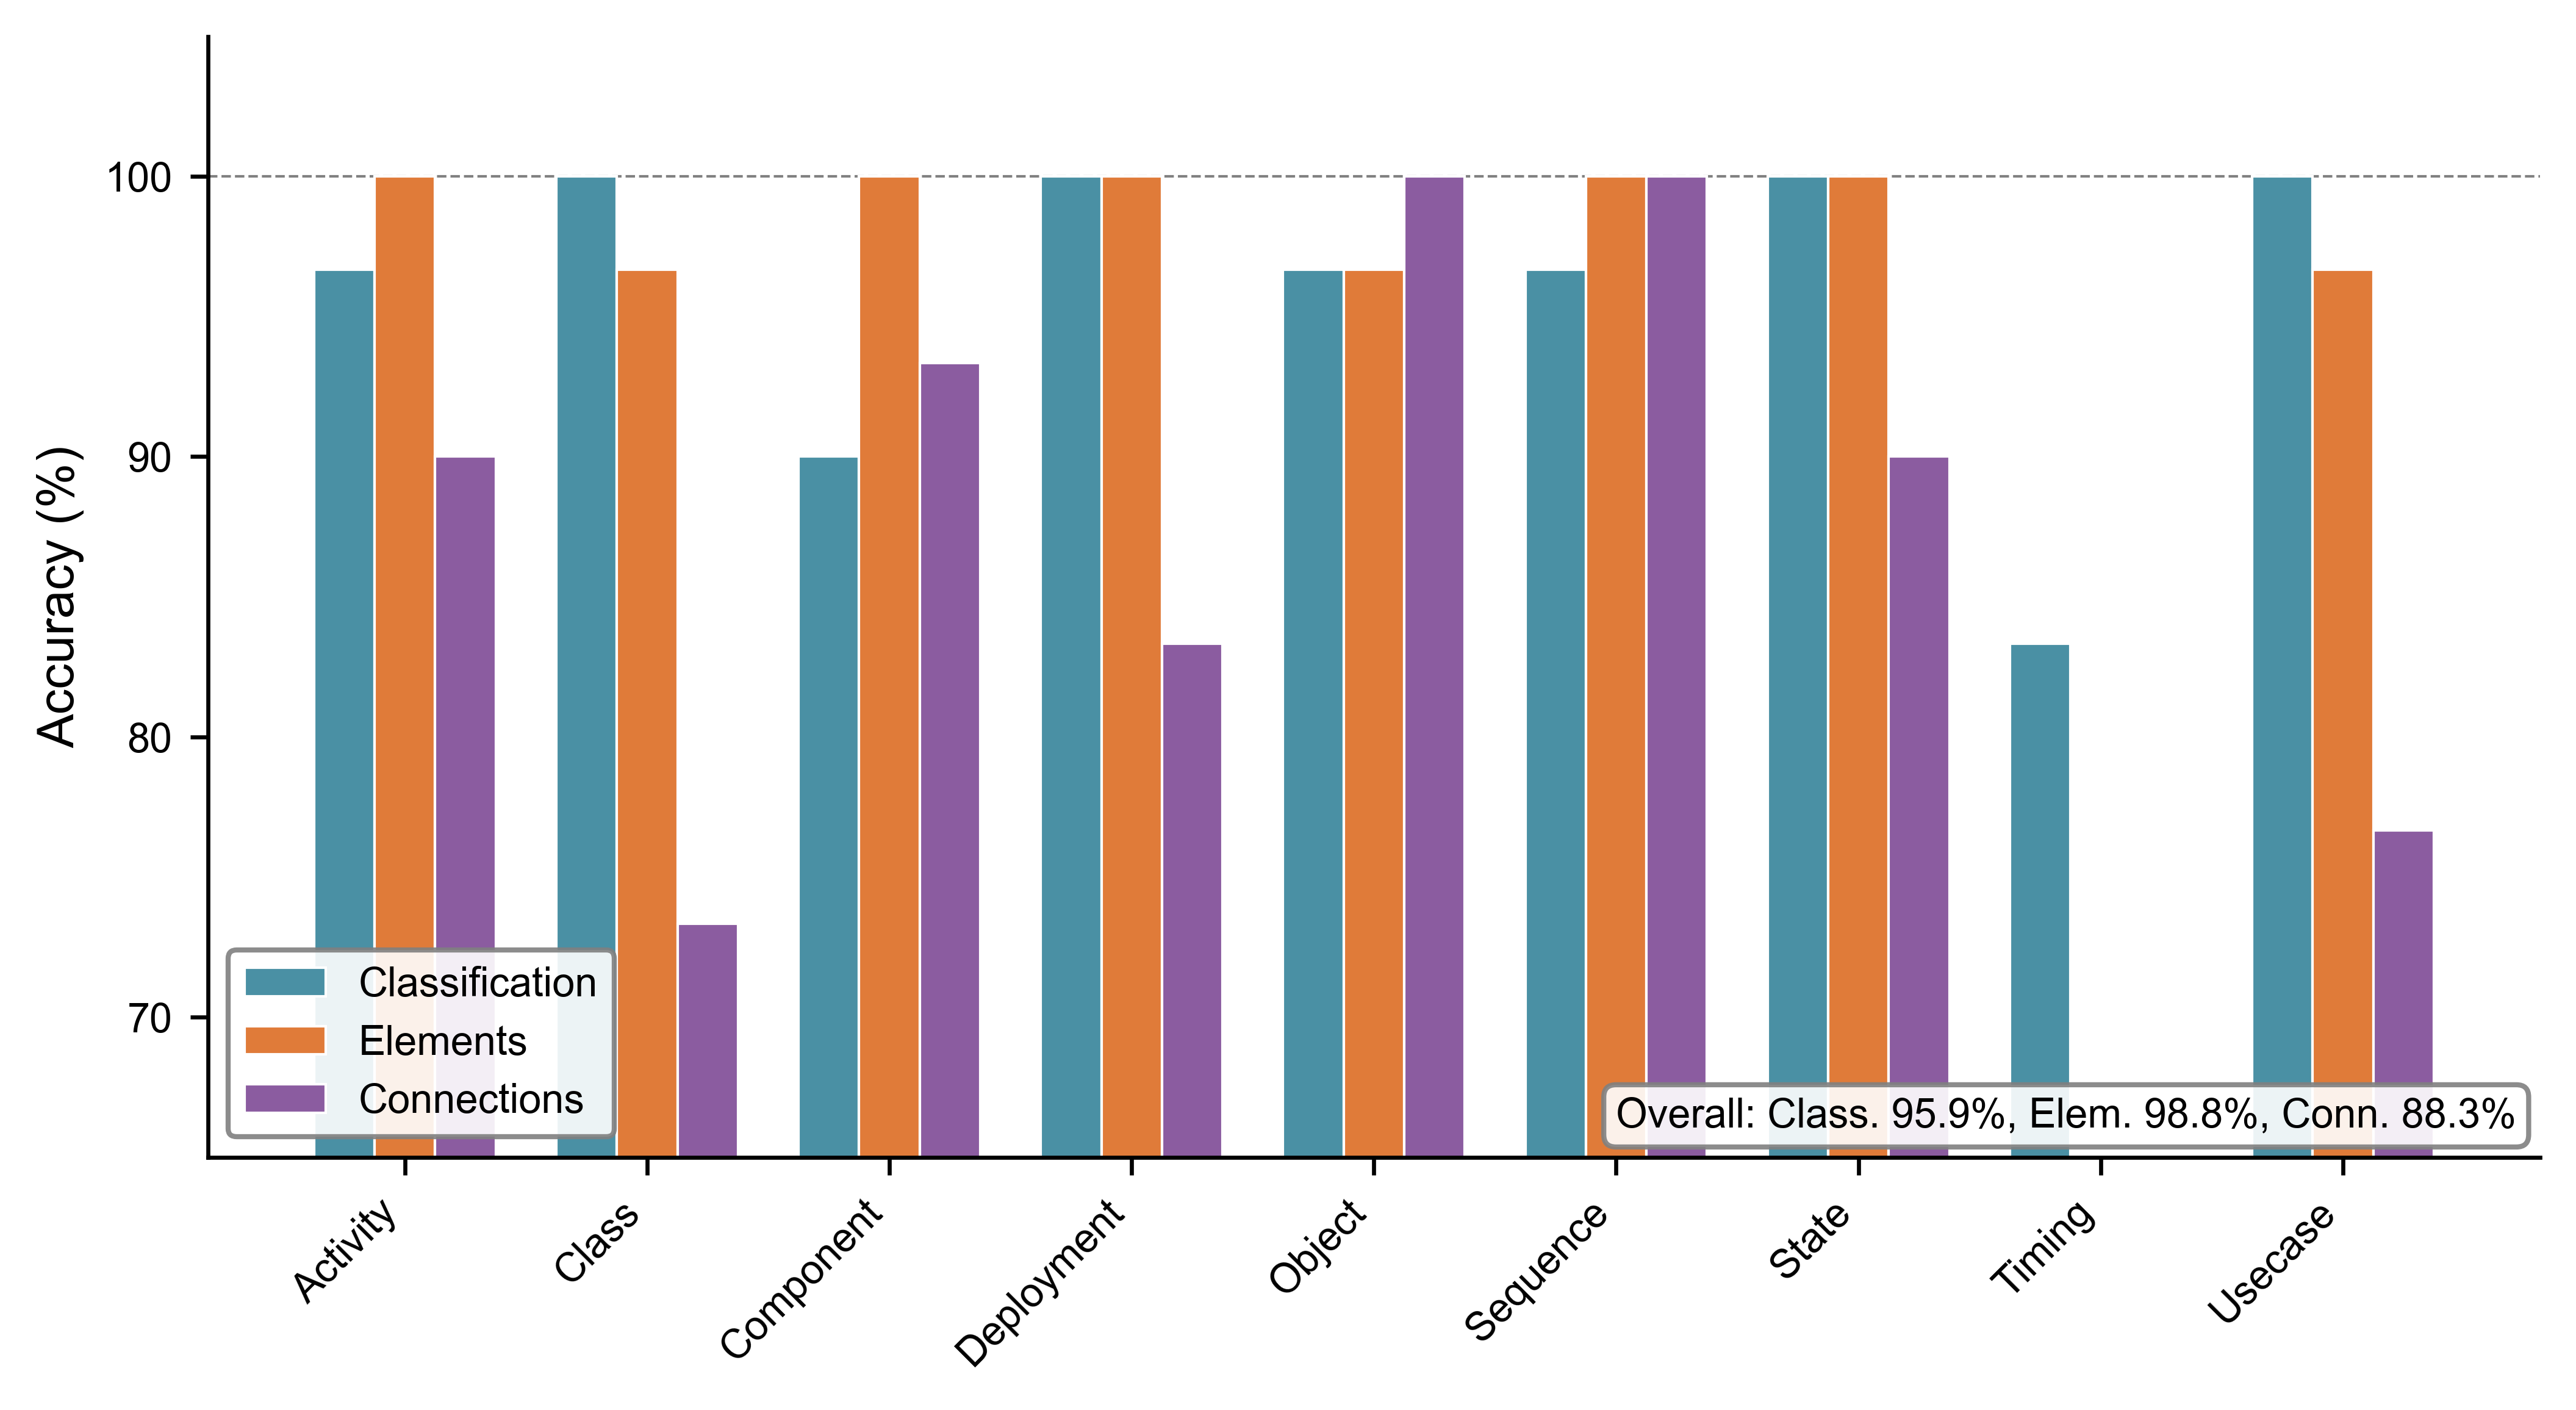
\includegraphics[width=\textwidth]{figures/fig6_validation_accuracy.png}
\caption{Per-type validation accuracy for classification, element extraction, and connection extraction (30~diagrams per type). Element and connection bars are absent for timing diagrams due to extraction limitations. A diagram counts as an exact match when both the per-type breakdown and the aggregate total agree with the expert review.\label{fig:validation-accuracy}}
\end{figure}

The 30~timing diagrams were excluded from element and connection validation because 178 of the 189~timing diagrams (94.2\%) in the full dataset have empty extraction fields (\texttt{unsupported\_type:TimingDiagram}). Classification accuracy for timing diagrams is 83.3\% (25/30), with all 5~errors being sequence diagrams that use the \texttt{!pragma teoz} syntax. Both identified connection biases are deterministic; downstream users can mitigate them by filtering \texttt{none}-type connections or consulting the \texttt{extraction\_error} metadata field.


%%%%%%%%%%%%%%%%%%%%%%%%%%%%%%%%%%%%%%%%%%
\section{User Notes}
\label{sec:usage-notes}

The metadata file (\texttt{uml\_metadata\_enriched.json}) can be loaded in Python with \texttt{json.load}. It contains three top-level keys: \texttt{metadata} records pipeline parameters (model identifier, timestamp, file counts); \texttt{statistics} provides pre-computed aggregate analytics---type distributions, element and connection summary statistics---so that users need not recompute these from individual records; and \texttt{classifications} contains one entry per diagram, keyed by filename.

The \texttt{repository} field uses the WoC project identifier convention, in which the first underscore separates the username from the repository name (e.g., \texttt{btratodos\_PracticeRepo}). For repositories hosted outside GitHub, the identifier is prefixed with the forge domain: \texttt{bitbucket.org\_user\_repo} or \texttt{gitlab.com\_user\_repo}. The corresponding repository URL can be constructed by replacing the forge prefix and first underscore with the appropriate base URL and path separator---for example, \texttt{GreenCape\_joomla-cli} maps to \url{https://github.com/GreenCape/joomla-cli}. Because both usernames and repository names may contain underscores, this reconstruction is ambiguous for some entries; users requiring exact URLs should consult the WoC API. The \texttt{original\_path} field provides the file path within the repository. As noted in Section~\ref{sec:metadata-schema}, 1,424 diagrams (1.0\%) have a \texttt{null} repository value due to incomplete WoC basemap coverage.

For most diagrams, the rendered PNG image shares the same base name as the source file (e.g., \texttt{5f95f42b...e89e.puml} and \texttt{5f95f42b...e89e.png}). Two exceptions apply: split diagrams, where a multi-diagram source was divided into individual files, follow the pattern \texttt{\{blob\_id\}\_01.puml} with a corresponding \texttt{\{blob\_id\}\_01.png}; and multi-page diagrams using PlantUML's \texttt{newpage} keyword produce multiple images from a single source, named \texttt{\{blob\_id\}\_001.png}, \texttt{\{blob\_id\}\_002.png}, etc. The \texttt{extraction\_error} field identifies 347~diagrams where the parser-based tool could not extract structural metrics, predominantly timing diagrams (\texttt{unsupported\_type:TimingDiagram}, 178) and multi-page diagrams (\texttt{unsupported\_type:NewpagedDiagram}, 167); users requiring complete element and connection counts should filter on this field. The \texttt{secondary\_types} array is non-empty for 983~diagrams that combine elements from multiple UML types; depending on the application, these may warrant separate treatment.

The dataset is released under the CC-BY-4.0 license, which covers the compiled metadata, rendered PNG images, and preprocessed PlantUML files. However, the PlantUML source files originate from open-source repositories whose individual licenses vary. Users who redistribute or build upon specific diagrams beyond the scope of research use should verify the license of the originating repository.

We anticipate several lines of reuse for this dataset: empirical studies of how UML is used in practice across the open-source ecosystem; training and evaluation of AI models for diagram classification, understanding, and generation---both from source code and from rendered images; benchmarking diagram-to-code and code-to-diagram translation tools; analysis of diagram structural complexity and quality; and development of educational resources that draw on real-world examples across all nine UML diagram types.


%%%%%%%%%%%%%%%%%%%%%%%%%%%%%%%%%%%%%%%%%%
\vspace{6pt}

%%%%%%%%%%%%%%%%%%%%%%%%%%%%%%%%%%%%%%%%%%
\authorcontributions{Conceptualization, V.P.; methodology, V.P.; software, V.P.; validation, V.P.; formal analysis, V.P.; data curation, V.P.; writing---original draft preparation, V.P.; writing---review and editing, Y.Y.; supervision, Y.Y. All authors have read and agreed to the published version of the manuscript.}

\funding{This research received no external funding.}

\institutionalreview{Not applicable.}

\informedconsent{Not applicable.}

\dataavailability{The dataset is openly available on Zenodo at \url{https://doi.org/10.5281/zenodo.18952372} under the CC-BY-4.0 license. It contains 143,427 PlantUML source files, 144,487 rendered PNG images, and a JSON metadata file with per-diagram classification and structural metrics. The extraction pipeline source code is available at \url{https://doi.org/10.5281/zenodo.19298761}. The element and connection extraction tool (DiagramStatsExtractor) is available at \url{https://doi.org/10.5281/zenodo.19288003}.}

\acknowledgments{The authors thank the World of Code team at the University of Tennessee, Knoxville, for providing access to the WoC infrastructure used for data extraction. During the preparation of this work, the authors used Claude (Anthropic) for automated diagram type classification (Claude Haiku~4.5) and for assistance with manuscript drafting and editing. The authors have reviewed and edited all AI-generated outputs and take full responsibility for the content of this publication.}

\conflictsofinterest{The authors declare no conflicts of interest.}

%%%%%%%%%%%%%%%%%%%%%%%%%%%%%%%%%%%%%%%%%%
\abbreviations{Abbreviations}{
The following abbreviations are used in this manuscript:
\\

\noindent
\begin{tabular}{@{}ll}
UML   & Unified Modeling Language \\
WoC   & World of Code \\
LLM   & Large Language Model \\
API   & Application Programming Interface \\
DOI   & Digital Object Identifier \\
SHA-1 & Secure Hash Algorithm 1 \\
PNG   & Portable Network Graphics \\
\end{tabular}
}

%%%%%%%%%%%%%%%%%%%%%%%%%%%%%%%%%%%%%%%%%%
%\isPreprints{}{% This command is only used for ``preprints''.
\begin{adjustwidth}{-\extralength}{0cm}
%} % If the paper is ``preprints'', please uncomment this parenthesis.

\reftitle{References}

%=====================================
% References: external bibliography
%=====================================
% \bibliography{references}

%=====================================
% References: internal bibliography
%=====================================
\begin{thebibliography}{999}

\bibitem{ma2021world}
Ma,~Y.; Dey,~T.; Bogart,~C.; Amreen,~S.; Valiev,~M.; Tutko,~A.; Kennard,~D.; Zaretzki,~R.L.; Mockus,~A. World of Code: Enabling a Research Workflow for Mining and Analyzing the Universe of Open Source VCS Data. {\em Empir. Softw. Eng.} {\bf 2021}, {\em 26}, 22. \url{https://doi.org/10.1007/s10664-020-09905-9}

\bibitem{petre2013uml}
Petre,~M. UML in Practice. In Proceedings of the 35th International Conference on Software Engineering (ICSE), San Francisco, CA, USA, 18--26 May 2013; pp. 722--731. \url{https://doi.org/10.1109/ICSE.2013.6606618}

\bibitem{reggio2014who}
Reggio,~G.; Leotta,~M.; Ricca,~F. Who Knows/Uses What of the UML: A Personal Opinion Survey. In Proceedings of the 17th International Conference on Model Driven Engineering Languages and Systems (MODELS), Valencia, Spain, 28 September--3 October 2014; pp. 149--165. \url{https://doi.org/10.1007/978-3-319-11653-2_10}

\bibitem{hoquang2017practices}
Ho-Quang,~T.; Hebig,~R.; Robles,~G.; Chaudron,~M.R.V.; Fern\'{a}ndez,~M.A. Practices and Perceptions of UML Use in Open Source Projects. In Proceedings of the IEEE/ACM 39th International Conference on Software Engineering: Software Engineering in Practice Track (ICSE-SEIP), Buenos Aires, Argentina, 20--28 May 2017; pp. 203--212. \url{https://doi.org/10.1109/ICSE-SEIP.2017.28}

\bibitem{karasneh2013img2uml}
Karasneh,~B.; Chaudron,~M.R.V. Online Img2UML Repository: An Online Repository for UML Models. In Proceedings of the 3rd International Workshop on Experiences and Empirical Studies in Software Modeling (EESSMod), Miami, FL, USA, 1 October 2013; pp. 61--66.

\bibitem{hebig2016quest}
Hebig,~R.; Ho-Quang,~T.; Chaudron,~M.R.V.; Robles,~G.; Fern\'{a}ndez,~M.A. The Quest for Open Source Projects That Use UML: Mining GitHub. In Proceedings of the ACM/IEEE 19th International Conference on Model Driven Engineering Languages and Systems (MODELS), Saint-Malo, France, 2--7 October 2016; pp. 173--183. \url{https://doi.org/10.1145/2976767.2976778}

\bibitem{robles2017extensive}
Robles,~G.; Ho-Quang,~T.; Hebig,~R.; Chaudron,~M.R.V.; Fern\'{a}ndez,~M.A. An Extensive Dataset of UML Models in GitHub. In Proceedings of the 14th International Conference on Mining Software Repositories (MSR), Buenos Aires, Argentina, 20--21 May 2017; pp. 519--522. \url{https://doi.org/10.1109/MSR.2017.48}

\bibitem{robles2023reflection}
Robles,~G.; Chaudron,~M.R.V.; Jolak,~R.; Hebig,~R. A Reflection on the Impact of Model Mining from GitHub. {\em Inf. Softw. Technol.} {\bf 2023}, {\em 164}, 107317. \url{https://doi.org/10.1016/j.infsof.2023.107317}

\bibitem{romeo2025uml}
Romeo,~J.; Raglianti,~M.; Nagy,~C.; Lanza,~M. UML Is Back. Or Is It? Investigating the Past, Present, and Future of UML in Open Source Software. In Proceedings of the 47th International Conference on Software Engineering (ICSE), Ottawa, ON, Canada, 27 April--3 May 2025; pp. 2342--2354. \url{https://doi.org/10.1109/ICSE55347.2025.00155}

\bibitem{storrle2014index}
St\"{o}rrle,~H.; Hebig,~R.; Knapp,~A. An Index for Software Engineering Models. In Proceedings of the Joint MODELS 2014 Poster Session and ACM Student Research Competition, Valencia, Spain, 28 September--3 October 2014; pp. 36--40.

\bibitem{groundtruth2024}
Torcal,~J.; Moreno,~V.; Llorens,~J.; Granados,~A. Creating and Validating a Ground Truth Dataset of Unified Modeling Language Diagrams Using Deep Learning Techniques. {\em Appl. Sci.} {\bf 2024}, {\em 14}, 10873. \url{https://doi.org/10.3390/app142310873}

\bibitem{gosala2021classification}
Gosala,~B.; Chowdhuri,~S.R.; Singh,~J.; Gupta,~M.; Mishra,~A. Automatic Classification of UML Class Diagrams Using Deep Learning Technique: Convolutional Neural Network. {\em Appl. Sci.} {\bf 2021}, {\em 11}, 4267. \url{https://doi.org/10.3390/app11094267}

\bibitem{bates2025umlcodegen}
Bates,~A.; Vavricka,~R.; Carleton,~S.; Shao,~R.; Pan,~C. Unified Modeling Language Code Generation from Diagram Images Using Multimodal Large Language Models. {\em Mach. Learn. Appl.} {\bf 2025}, {\em 20}, 100660. \url{https://doi.org/10.1016/j.mlwa.2025.100660}

\bibitem{camara2024image}
Conrardy,~A.; Cabot,~J. From Image to UML: First Results of Image-Based UML Diagram Generation Using LLMs. In Proceedings of the LLM4MDE Workshop at STAF 2024, Enschede, The Netherlands, 8--11 July 2024; pp. 55--65.

\bibitem{pfdial2025}
Zhang,~M.; Wang,~Y.; Shen,~Y.; Yang,~T.; Jiang,~C.; Wu,~Y.; Dou,~S.; Chen,~Q.; Xi,~Z.; Zhang,~Z.; Dong,~Y.; Wang,~Z.; Fei,~Z.; Wan,~M.; Liang,~T.; Ma,~G.; Zhang,~Q.; Gui,~T.; Huang,~X. PFDial: A Structured Dialogue Instruction Fine-Tuning Method Based on UML Flowcharts. In Findings of the Association for Computational Linguistics: ACL 2025, Vienna, Austria, 2025; pp. 2626--2649. \url{https://doi.org/10.18653/v1/2025.findings-acl.134}

\end{thebibliography}

%%%%%%%%%%%%%%%%%%%%%%%%%%%%%%%%%%%%%%%%%%
\PublishersNote{}
%\isPreprints{}{% This command is only used for ``preprints''.
\end{adjustwidth}
%} % If the paper is ``preprints'', please uncomment this parenthesis.
\end{document}
